%% evenend-theory-ja.tex：evenendパッケージの定式化（マクロタイポグラフィの要請，問題の定義，
%% 手順，証明）
%% LuaLaTeXで2回組む．使い方はマニュアル（evenend-ja.tex）にある
%% この文書そのものを，evenendの見本として組む．1段を基本にして（columns=1），
%% 部分ごとにmulticols環境，evenendmulticols環境，\evenendcolumnsで段組にする
\documentclass[paper=a4,fontsize=10pt]{jlreq}
\usepackage{graphicx}
\usepackage{array}
\usepackage{tcolorbox}
\usepackage[columns=1]{evenend}
%% 段組の後，ページの残りが2行あれば，そのページに続きを組む（既定は5行）
\evenendsetup{blockmin=2\baselineskip}
\setlength\columnseprule{0pt}
%% ページの残りが2行あれば，そこから段組を始める（既定は50pt）．\premulticolsは，
%% evenendが文書の始まりで用意するので，その後で変える
\AtBeginDocument{\setlength\premulticols{2\baselineskip}}
\tcbset{colback=white,colframe=black!55,boxrule=.4pt,arc=1.5pt,
  left=1\zw,right=1\zw,top=.5\baselineskip,bottom=.5\baselineskip,
  before skip=.75\baselineskip,after skip=.75\baselineskip}
\usepackage{tikz}
\usetikzlibrary{arrows.meta,positioning,calc}
\tikzset{
  alg/.style={font=\small,>={Stealth[length=5pt]},node distance=5mm and 9mm},
  proc/.style={draw,rounded corners=2pt,align=left,inner sep=4pt,text width=#1},
  proc/.default=11\zw,
  cond/.style={draw,chamfered rectangle,chamfered rectangle xsep=6pt,align=center,inner sep=3pt,text width=#1},
  cond/.default=9\zw,
  term/.style={draw,rounded corners=8pt,align=center,inner sep=4pt,text width=#1},
  term/.default=9\zw,
  lab/.style={font=\footnotesize,inner sep=1.5pt},
}
\usetikzlibrary{shapes.misc}
\usepackage{hyperref}
\hypersetup{hidelinks,pdftitle={evenendパッケージの定式化},pdfauthor={木枝祐介}}

%% ロゴ（クラスやパッケージが定義していなければ定義する）
\providecommand\LuaTeX{Lua\TeX}
\providecommand\LuaLaTeX{Lua\LaTeX}
\newcommand\cs[1]{\texttt{\textbackslash #1}}
%% 制御綴の「\」と和文の間にも和欧文間のアキを入れる（LuaTeX-jaの既定では入らない）
\ltjsetparameter{alxspmode={`\\,allow}}
\newcommand\opt[1]{\texttt{#1}}
\newcommand\pkg[1]{\textsf{#1}}
%% 強調：和文はゴシック体，欧文はイタリック体
\newcommand\kyocho[1]{{\gtfamily\itshape #1}}
%% 例の図：x=1mm，y=-.25mm（縦は1ptを0.25mmとし，下向き）で描く
%% \excol[高さ]{x}{y}：段の地，\exlines{x}{1行目のベースライン}{行数}：本文の行，
%% \exfloat{x}{y}：フロート（40ptと下のアキ8pt），\exfoot{x}{最終行のベースライン}：脚注
\newcommand\excol[3][178]{\fill[black!8] (#2,#3) rectangle ++(20,#1);}
\newcommand\exlines[3]{\foreach \exi in {1,...,#3}
  {\fill[black!18] (#1,{#2+(\exi-1)*12-7}) rectangle ++(20,7);}}
\newcommand\exfloat[2]{\fill[black!45] (#1,#2) rectangle ++(20,40);}
\newcommand\exfoot[2]{\draw[line width=.3pt] (#1,{#2-12}) -- ++(7,0);
  \fill[black!30] (#1,{#2-5}) rectangle ++(20,5);}
%% 定義・問題・命題などの文：\begin{stmt}[名前]{種類}
\newcounter{stmt}
\newenvironment{stmt}[2][]{%
  \par\addvspace{.5\baselineskip}\refstepcounter{stmt}%
  \noindent{\gtfamily\sffamily #2\thestmt}%
  \if\relax\detokenize{#1}\relax\else （#1）\fi\hspace{1\zw}\ignorespaces}
  {\par\addvspace{.5\baselineskip}}
%% 手順（文の主張する手順そのもの）と証明
\newenvironment{tejun}{%
  \par\noindent{\gtfamily\sffamily 手順}\hspace{1\zw}\ignorespaces}
  {\par\addvspace{.5\baselineskip}}
\newenvironment{shoumei}{%
  \par\noindent{\gtfamily\sffamily 証明}\hspace{1\zw}\ignorespaces}
  {\unskip\nobreak\hfill □\par\addvspace{.5\baselineskip}}
%% その場に置く図（フロートにしない）：例の図など，文のすぐ後に置きたい図に使う．段組や箱の中でも使える
\makeatletter
\newenvironment{zu}{\par\addvspace{.75\baselineskip}\noindent
  \begin{minipage}{\linewidth}\def\@captype{figure}\centering}
  {\end{minipage}\par\addvspace{.75\baselineskip}}
\makeatother
%% 要請の項目（段組の中で使う）：\yousei{番号}{観点}
\newcommand\yousei[2]{\par\noindent(M#1)\hspace{.5\zw}\kyocho{#2}．\ignorespaces}
%% 対応の一覧の項目（表の代わり）：\taiou{左の欄}{中の欄}
\newcommand\taiou[2]{\par\addvspace{.3\baselineskip}\noindent
  {\gtfamily\sffamily #1}\par\nobreak
  {\raggedright\hangindent=2.5\zw\hangafter=1\noindent\hspace{1\zw}→\hspace{.5\zw}#2\par}\nobreak\noindent\ignorespaces}
%% 組み方の設定の注記：その部分の最後に小さく記す．\settei[見出し]{設定}
\newcommand\settei[2][この段組の設定]{\par\nobreak\vspace{.25\baselineskip}%
  {\raggedright\footnotesize\noindent［#1：#2］\par}}
%% フロートにした図の設定の注記（キャプションの下に置く）
\newcommand\setteizu[1]{\par\vspace{.25\baselineskip}{\footnotesize［この図の設定：#1］\par}}
%% 地の文の小見出し
\newcommand\komidashi[1]{\par\addvspace{.5\baselineskip}%
  \noindent{\gtfamily\sffamily #1}\hspace{1\zw}\ignorespaces}

\title{\pkg{evenend}パッケージの定式化\\[.5\baselineskip]
  \large マクロタイポグラフィの要請，問題，手順，証明}
\author{木枝祐介}
\date{v20261126.0}

\begin{document}
\maketitle

\begin{multicols}{2}
evenendパッケージは，段組の紙面の構成を決め直す．行の中の組み（マイクロタイポグラフィ）には
触れず，組み上がった行，図表，脚注を，段と版面のどこに置くか（マクロタイポグラフィ）
だけを扱う．この文書では，その判断を定式化する．まず，紙面の構成についての要請を
言葉で立てる（\ref{sec:f-req}節）．次に，要請を式の条件に置き換えて問題を定義し
（\ref{sec:f-structure}節から\ref{sec:f-even}節），解を作る手順とその性質の証明を，実装
（\texttt{evenend.lua}の\texttt{balance}）に即して記す（\ref{sec:f-proc}節）．終わりに，
要請のそれぞれについて，証明できたことと，できていないことをまとめる
（\ref{sec:f-summary}節）．

要請の意味と，それを選んだ理由は，\texttt{evenend-typography-ja.pdf}（「\pkg{evenend}
パッケージの組版」）に述べてある．使い方はマニュアル（\texttt{evenend-ja.pdf}）を
参照されたい．マニュアルの「揃え方」と「仕組み」の節とは，内容は同じで，述べ方だけが違う．

長さはすべて段の上端から下向きに測る．記号が\TeX{}のどの概念（\cs{box}255，インサート，
マークなど）にあたるかは，\ref{sec:formal-tex}節にまとめる．証明の一部は，定理証明支援系
Lean 4でも確かめてある（\ref{sec:lean}節）．
\settei{\texttt{\cs{begin}\{multicols\}\{2\}}}
\end{multicols}

\komidashi{この文書の組み方}
この文書そのものを，\pkg{evenend}の見本として組んでいる．1段を基本にして，部分ごとに
段組にする．組み方を変えた部分の設定は，それぞれの最後に小さく記した．同じ設定の2段の
\texttt{multicols}環境が続く所では，節ごとに最初の1つにだけ記してある．文書全体の設定は，
文書の最後に記した．どの機能がどこにあるかは，次のとおりである．
\begin{evenendmulticols}[columnsep=2\zw,columnseprule=.4pt]{2}
\begin{itemize}
  \item 2段の\texttt{multicols}環境：始めの文，例\ref{ex:used}（\pageref{ex:used}ページ）
    などの例，証明，注意\ref{rem:noproof}．
  \item 3段で，前置きのある\texttt{multicols}環境：\ref{sec:f-req}節．見出しと始めの文が
    前置きで，全幅に組まれる．
  \item \texttt{evenendmulticols}環境で段間と段間罫を変えた段組：この項目の並び，
    例\ref{ex:material}，注意\ref{rem:exist}，\ref{sec:f-summary}節（前置きつき）．
  \item \cs{columnbreak}：例\ref{ex:material}（\pageref{ex:material}ページ）．文と図を段に
    分ける．
  \item \pkg{tcolorbox}の箱の中の段組：問題\ref{prob:main}（\pageref{prob:main}ページ）．
  \item \texttt{minipage}の中の段組：\ref{sec:formal-apply}節の「箱の中の段組」の項
    （\pageref{par:nest}ページ）．
  \item 段組の中の脚注：\ref{sec:formal-tex}節（\pageref{fn:whatsit}ページ）．脚注は
    版面の下端に全幅で置かれる（\opt{footnote=page}）．
  \item \cs{evenendcolumns}による切り換え：\ref{sec:lean}節から終わりまでは2段．最終
    ページで段の下端が揃う．
  \item フロートの図（\texttt{figure}環境）：図\ref{fig:formal-layout}，図\ref{fig:formal-even}，
    図\ref{fig:formal-fill}から図\ref{fig:formal-tex}．ほかの図は，その場に置いてある．
  \item 表の代わりの項目の並び：\ref{sec:formal-tex}節と\ref{sec:lean}節の対応の一覧は，
    段組に流してある．
\end{itemize}
\settei{\texttt{\cs{begin}\{evenendmulticols\}[columnsep=2\cs{zw},\allowbreak columnseprule=.4pt]\{2\}}}
\end{evenendmulticols}

\begin{multicols}{3}[\section{マクロタイポグラフィの要請}\label{sec:f-req}%
段組の本文がページの途中で終わるとき，\LaTeX{}は左の段から詰めて組む（なりゆき）．
evenendは，これを，各段の下端の揃った紙面に組み直す．このとき紙面に求めることを，
観点ごとに挙げる．]
\yousei{1}{構造}紙面の基準を動かさない．横の基準は段（段数，段幅，
    段間），縦の基準は行の位置（1行目のベースラインから行送りごとの位置）である．
\yousei{2}{版面}どの段も，版面の中で段組に使える高さを超えない．
\yousei{3}{読む順序}本文の順を変えない．図表の番号の順を変えず，
    図表を前の段へ動かさない．
\yousei{4}{配置}脚注は，参照する箇所と同じ段の下端か，版面の下端に
    全幅で置く．上の図表は段の上端に，下の図表は段の下端に置く．
\yousei{5}{釣り合い}中身のある最後の段を除いて，段の下端を1つの
    位置に揃える．最後の段は，その位置より下に出ない．
\yousei{6}{整列}段の下端は，目に見える下端で測る．下端を揃える
    ために，本文の行を行の位置から動かさない．
\yousei{7}{余白}段組をできるだけ低くして，余白を段組の下に
    まとめる．高さを合わせるためのアキは，行間に入れず，本文と図表，本文と脚注の境に
    入れる．
\yousei{8}{一貫性}図表は，\LaTeX{}が置いた段からなるべく動かさない．
    ページの途中で段組を改めるときも，ほかのページを組み直すときも，同じ手順を使う．
\settei{\texttt{\cs{begin}\{multicols\}\{3\}[前置き]}．前置きは，節の見出しと始めの文}
\end{multicols}
横の基準は，この文書の式には現れない．段幅と段間は初めに決まり，本文の行と図表は
その幅で組み上がっているので，決め直すのは縦の方向だけである．以下では，材料の高さと，
それを段に分ける位置だけを扱う．

要請は，互いにぶつかることがある．行も図表も分けられないので，(M6)を守ると(M5)が
満たせないことがある．どちらを先に守るかは，問題の条件の立て方（問題\ref{prob:main}）と
手順の順（命題\ref{prop:main}）に表れる．

\section{構造：段組と材料}\label{sec:f-structure}

紙面の構造（M1）を，段数$N$，行送り$b$，1行目のベースラインの位置$\tau$で表す．行の位置は
$\tau+\ell b$（$\ell=0,1,\dots$）である．版面（M2）は，段の高さ$H$で表す．段に入れる
ものは，本文，段内フロート，脚注の3つで，これを材料と呼ぶ．

\begin{stmt}[段組]{定義}\label{def:frame}
段数を$N\ge 1$，段の高さを$H$，行送りを$b$（\cs{baselineskip}），1行目のベースラインの
位置を$\tau$（\cs{topskip}）とする．$H$は，版面の高さから，段抜きのフロート，そのページに
すでに積んだ段組とその後のアキを除いた高さ（\cs{@colht}）である
（図\ref{fig:formal-frame}の左）．
\end{stmt}

図\ref{fig:formal-frame}の左で，段の高さ$H$は，版面の高さから，段抜きのフロート，すでに
積んだ段組，その後のアキを除いた高さである（ごく薄い地が段）．右は，定義\ref{def:used}で
定める所要の高さを示す．段$i$の所要の高さ$U_i$は，フロートの高さ$|F_i|$（まわりのアキを
含む），本文の高さ$|T_i|$，脚注の高さ$G_i$（区切りの罫と上のアキを含む）の和である．
どの段でも$U_i\le h$なら，配置は$h$に入り切る．

\begin{zu}
  \begin{tikzpicture}[alg,x=.9mm,y=.9mm,
      txt/.style={fill=black!18},fl/.style={fill=black!45}]
    %% ページの中の段組
    \draw (0,0) rectangle (50,70);
    \node[lab,above] at (25,70) {版面};
    \fill[fl] (0,62) rectangle (50,70);
    \node[lab,text=white] at (25,66) {段抜きのフロート};
    \foreach \i in {0,...,2} {\fill[txt] (0,59-3*\i) rectangle (23,57.2-3*\i);
      \fill[txt] (27,59-3*\i) rectangle (50,57.2-3*\i);}
    \node[lab,left,align=right] at (-1,55) {すでに積んだ\\段組};
    \draw[|-|] (-2,50.5) -- node[lab,left] {アキ} (-2,46);
    \fill[black!8] (0,0) rectangle (23,46);
    \fill[black!8] (27,0) rectangle (50,46);
    \draw (0,0) rectangle (50,70);
    \node[lab] at (11.5,23) {段1};
    \node[lab] at (38.5,23) {段$N$};
    \draw[<->] (53,0) -- node[lab,right] {$H$} (53,46);
    %% 段iの中身
    \begin{scope}[xshift=70.2mm]
      \node[lab,above] at (17,70) {段$i$};
      \fill[fl] (0,60) rectangle (34,70);
      \node[lab,text=white] at (17,65) {上のフロート};
      \foreach \i in {0,...,6} \fill[txt] (0,55-4*\i) rectangle (34,52.8-4*\i);
      \draw[|-|] (-3,48.8) -- node[lab,left=4pt] {$b$} (-3,44.8);
      \draw (0,24) -- (12,24);
      \fill[txt] (0,20.4) rectangle (34,22);
      \fill[txt] (0,17) rectangle (22,18.6);
      \node[lab,left] at (-1,20) {脚注};
      \draw[densely dashed] (-6,12) -- (60,12);
      \draw (-6,0) -- (68,0);
      \draw[|-|] (37,70) -- node[lab,right] {$|F_i|$} (37,57);
      \draw[|-|] (37,57) -- node[lab,right] {$|T_i|$} (37,28.8);
      \draw[|-|] (37,28.8) -- node[lab,right] {$G_i$} (37,17);
      \draw[<->] (48,70) -- node[lab,right] {$U_i$} (48,17);
      \draw[<->] (56,70) -- node[lab,right,pos=.3] {$h$} (56,12);
      \draw[<->] (64,70) -- node[lab,right,pos=.2] {$H$} (64,0);
    \end{scope}
  \end{tikzpicture}
  \caption{段組と所要の高さ（定義\ref{def:frame}，\ref{def:used}）}
  \label{fig:formal-frame}
\end{zu}

\begin{stmt}[段組]{例}\label{ex:frame}
この節の例では，次の1つの段組を通して使う（図\ref{fig:ex-frame}）．段数は$N=3$，行送りは
$b=12\,\mathrm{pt}$，1行目のベースラインの位置は$\tau=10\,\mathrm{pt}$である．版面の高さは
$238\,\mathrm{pt}$で，上に段抜きのフロートがあり，下のアキを含めて$60\,\mathrm{pt}$を占める．
よって，段の高さは$H=238-60=178\,\mathrm{pt}$である．$178=\tau+14b$なので，1つの段に
本文が15行入る．
\end{stmt}

図\ref{fig:ex-frame}で，版面から段抜きのフロートとその下のアキを除いた高さが，段の
高さ$H$である（ごく薄い地が段）．


\begin{stmt}[材料]{定義}\label{def:material}
ページの\kyocho{材料}とは，次の3つの組$M=(T,F,\Phi)$である．
\begin{itemize}
  \item 本文$T=(t_1,\dots,t_n)$：\LaTeX{}が組んだ全段の本文を，読む順に1本につないだ垂直
    リスト．要素は，箱（行など），グルー，カーン，ペナルティである．改段の位置で\TeX{}が
    捨てたグルーは，元に戻してつなぐ．
  \item 段内フロートの列$F=(f_1,\dots,f_m)$：番号順に並べる．$f_j$は，高さ$|f_j|$（まわりの
    アキを含む），位置$\pi_j\in\{\mbox{上},\mbox{下}\}$，\LaTeX{}が置いた段$o_j\in\{1,\dots,N\}$を
    持つ．\LaTeX{}がまだ置いていない（持ち越した）フロートは$o_j=1$とする．
  \item 脚注の集合$\Phi$：脚注$\varphi$は，高さ$|\varphi|$と，参照位置の行$a(\varphi)\in
    \{1,\dots,n\}$を持つ．
\end{itemize}
\end{stmt}

%% 調整：図2は，ページの下の空きを詰めるために，例2の直後から定義3の後へ送ってある
\begin{zu}
  \begin{tikzpicture}[alg,x=1mm,y=-.25mm]
    \fill[black!45] (0,0) rectangle (68,48);
    \node[white] at (34,24) {段抜きのフロート};
    \foreach \x in {0,24,48} {\excol{\x}{60}}
    \foreach \x/\i in {10/1,34/2,58/3} {\node at (\x,149) {段\i};}
    \draw (0,0) rectangle (68,238);
    \draw[<->] (72,0) -- (72,60) node[midway,right=2pt] {$60\,\mathrm{pt}$（下のアキを含む）};
    \draw[<->] (72,60) -- (72,238) node[midway,right=2pt] {$H=178\,\mathrm{pt}$（15行）};
    \draw[<->] (-4,0) -- (-4,238) node[midway,left=2pt] {版面$238\,\mathrm{pt}$};
  \end{tikzpicture}
  \caption{例\ref{ex:frame}の段組}
  \label{fig:ex-frame}
\end{zu}

\begin{evenendmulticols}[columnsep=2\zw,columnseprule=.4pt]{2}
\begin{stmt}[材料]{例}\label{ex:material}
例\ref{ex:frame}の段組に，次の材料を組む（図\ref{fig:ex-material}）．
\begin{itemize}
  \item 本文$T$は23行で，行の間のグルーは行送りだけとする．以下，番号は行だけに振り，
    $T=(t_1,\dots,t_{23})$と書く．
  \item 段内フロートは$F=(f_1)$の1つで，高さ$|f_1|=48\,\mathrm{pt}$（下のアキを含む．
    $4b$にあたる），位置$\pi_1=\mbox{上}$である．\LaTeX{}は段1に置いた（$o_1=1$）．
  \item 脚注は$\Phi=\{\varphi\}$の1つで，参照位置は3行目（$a(\varphi)=3$）である．
    区切りの罫と上のアキを含めた塊の高さは$20\,\mathrm{pt}$とする．
\end{itemize}
本文の行の深さは，どの行も$d=3\,\mathrm{pt}$とする．
\end{stmt}
\columnbreak

図\ref{fig:ex-material}で，本文$T$は23行を1本につないだもの，$f_1$は段内フロート，
$\varphi$は3行目（\textdagger）に参照位置のある脚注である．

\begin{zu}
  \begin{tikzpicture}[alg,x=.7mm,y=-.18mm]
    \exlines{0}{10}{23}
    \node[left=2pt] at (0,6.5) {$t_1$};
    \node[left=2pt] at (0,30.5) {$t_3$};
    \node[left=2pt] at (0,270.5) {$t_{23}$};
    \node[font=\footnotesize] at (17,30.5) {\textdagger};
    \node at (10,298) {本文$T$};
    \exfloat{40}{0}
    \draw[<->] (63,0) -- (63,48) node[midway,right=2pt] {$|f_1|=48\,\mathrm{pt}$};
    \draw[densely dotted] (60,48) -- (64,48);
    \node[anchor=west] at (38,72) {フロート$f_1$（上，$o_1=1$）};
    \exfoot{40}{120}
    \draw[<->] (63,100) -- (63,120) node[midway,right=2pt] {$20\,\mathrm{pt}$};
    \node[anchor=west] at (38,146) {脚注$\varphi$（$a(\varphi)=3$）};
    \draw[->,densely dashed] (20,30.5) to[out=0,in=180] (30,80) to[out=0,in=180] (39,112);
  \end{tikzpicture}
  \caption{例\ref{ex:material}の材料}
  \label{fig:ex-material}
\end{zu}
\settei{\texttt{\cs{begin}\{evenendmulticols\}[columnsep=2\cs{zw},\allowbreak columnseprule=.4pt]\{2\}}．文と図の間に\texttt{\cs{columnbreak}}}
\end{evenendmulticols}

\section{配置と読む順序}\label{sec:f-layout}

材料を段に分けたものを，配置と呼ぶ．読む順序（M3）は，配置の定義の中に組み込む．本文は
切れ目で分けるだけにして順を変えず，フロートの割り振りには，番号の順を保つことと，前の
段へ動かさないことを条件として課す．

%% 調整：図4は，参照するページに入るように，3節の始めに置いてある
\begin{figure}[tbp]
  \centering
  \begin{tikzpicture}[alg,x=.9mm,y=.9mm,
      txt/.style={fill=black!18},fl/.style={fill=black!45}]
    %% 材料：フロートFと本文T
    \node[lab,above] at (-30,61) {フロート$F$};
    \fill[fl] (-36,48) rectangle (-24,56);
    \node[lab,text=white] at (-30,52) {$f_1$};
    \fill[fl] (-36,34) rectangle (-24,42);
    \node[lab,text=white] at (-30,38) {$f_2$};
    \node[lab,below,align=center] at (-30,33) {$o_1=1$\\$o_2=2$};
    \node[lab,above] at (6,61) {本文$T$};
    \foreach \i in {0,...,19} \fill[txt] (0,60-3*\i) rectangle (12,58.2-3*\i);
    \foreach \y/\t in {60.6/{$k_0=0$},39.6/{$k_1$},18.6/{$k_2$},0.6/{$k_3=n$}}
      {\draw (-2,\y) -- (14,\y); \node[lab,left] at (-2,\y) {\t};}
    \draw[|-|] (17,60) -- node[lab,right] {$T_1$} (17,40.2);
    \draw[|-|] (17,39) -- node[lab,right] {$T_2$} (17,19.2);
    \draw[|-|] (17,18) -- node[lab,right] {$T_3$} (17,1.2);
    \draw[->] (28,30) -- node[lab,above,align=center] {配置\\$(k,s)$} (42,30);
    %% 配置
    \begin{scope}[xshift=43.2mm]
      \foreach \c/\t in {0/段1,24/段2,48/段3} \node[lab,above] at (\c+9,61) {\t};
      \fill[fl] (0,52) rectangle (18,60);
      \node[lab,text=white] at (9,56) {$f_1$};
      \foreach \i in {0,...,6} \fill[txt] (0,50-3*\i) rectangle (18,48.2-3*\i);
      \node[lab,below] at (9,29.5) {$T_1$};
      \foreach \i in {0,...,6} \fill[txt] (24,60-3*\i) rectangle (42,58.2-3*\i);
      \node[lab,below] at (33,39.5) {$T_2$};
      \fill[fl] (48,52) rectangle (66,60);
      \node[lab,text=white] at (57,56) {$f_2$};
      \foreach \i in {0,...,5} \fill[txt] (48,50-3*\i) rectangle (66,48.2-3*\i);
      \node[lab,below] at (57,32.5) {$T_3$};
      \node[lab,below,align=center] at (9,22) {$s(1)=1$\\（$=o_1$）};
      \node[lab,below,align=center] at (57,22) {$s(2)=3$\\（$>o_2$．後ろの段へ）};
    \end{scope}
  \end{tikzpicture}

  \vspace{\baselineskip}
  \begin{tikzpicture}[alg,x=.9mm,y=.9mm,
      txt/.style={fill=black!18},fl/.style={fill=black!45}]
    \node[lab,align=left,anchor=west] at (-38,10) {$N=2$，$m=2$，\\$o=(1,1)$の\\ときの$S$};
    %% σ=(1,1)
    \begin{scope}
      \fill[fl] (0,16) rectangle (9,21); \node[lab,text=white] at (4.5,18.5) {1};
      \fill[fl] (0,10) rectangle (9,15); \node[lab,text=white] at (4.5,12.5) {2};
      \foreach \i in {0,...,2} \fill[txt] (0,8-3*\i) rectangle (9,6.5-3*\i);
      \foreach \i in {0,...,6} \fill[txt] (11,20-3*\i) rectangle (20,18.5-3*\i);
      \node[lab,below,align=center] at (10,-1) {$s=(1,1)$\\$\mu=0$};
    \end{scope}
    %% σ=(1,2)
    \begin{scope}[xshift=30.6mm]
      \fill[fl] (0,16) rectangle (9,21); \node[lab,text=white] at (4.5,18.5) {1};
      \foreach \i in {0,...,4} \fill[txt] (0,14-3*\i) rectangle (9,12.5-3*\i);
      \fill[fl] (11,16) rectangle (20,21); \node[lab,text=white] at (15.5,18.5) {2};
      \foreach \i in {0,...,4} \fill[txt] (11,14-3*\i) rectangle (20,12.5-3*\i);
      \node[lab,below,align=center] at (10,-1) {$s=(1,2)$\\$\mu=1$};
    \end{scope}
    %% σ=(2,2)
    \begin{scope}[xshift=61.2mm]
      \foreach \i in {0,...,6} \fill[txt] (0,20-3*\i) rectangle (9,18.5-3*\i);
      \fill[fl] (11,16) rectangle (20,21); \node[lab,text=white] at (15.5,18.5) {1};
      \fill[fl] (11,10) rectangle (20,15); \node[lab,text=white] at (15.5,12.5) {2};
      \foreach \i in {0,...,2} \fill[txt] (11,8-3*\i) rectangle (20,6.5-3*\i);
      \node[lab,below,align=center] at (10,-1) {$s=(2,2)$\\$\mu=2$};
    \end{scope}
    %% σ=(2,1)：番号順に反する
    \begin{scope}[xshift=91.8mm]
      \fill[fl] (0,16) rectangle (9,21); \node[lab,text=white] at (4.5,18.5) {2};
      \foreach \i in {0,...,4} \fill[txt] (0,14-3*\i) rectangle (9,12.5-3*\i);
      \fill[fl] (11,16) rectangle (20,21); \node[lab,text=white] at (15.5,18.5) {1};
      \foreach \i in {0,...,4} \fill[txt] (11,14-3*\i) rectangle (20,12.5-3*\i);
      \draw[thick] (-2,-1) -- (22,23) (-2,23) -- (22,-1);
      \node[lab,below,align=center] at (10,-1) {$s=(2,1)$\\番号順に反する};
    \end{scope}
  \end{tikzpicture}
  \caption{材料と配置（定義\ref{def:material}，\ref{def:layout}）}
  \label{fig:formal-layout}
  \setteizu{\texttt{\cs{begin}\{figure\}[tbp]}}
\end{figure}

\begin{stmt}[配置]{定義}\label{def:layout}
材料$M$の\kyocho{配置}とは，次の組$(k,s)$である（図\ref{fig:formal-layout}）．
\begin{itemize}
  \item 切れ目$k=(k_0,\dots,k_N)$，$0=k_0\le k_1\le\dots\le k_N=n$．段$i$の本文は
    $T_i=(t_{k_{i-1}+1},\dots,t_{k_i})$である．切れ目は，\TeX{}が改ページできる位置に限る．
    段の先頭に来た捨てられる要素（グルーなど）は，$T_i$から除く．
  \item フロートの割り振り$s\colon\{1,\dots,m\}\to\{1,\dots,N\}$．次の2つを満たす．
    \begin{enumerate}
      \item 番号順を保つ：$s(j)\le s(j+1)$．
      \item 前の段へ動かさない：$s(j)\ge o_j$．段をまたぐフロートは$s(j)=o_j$．
    \end{enumerate}
\end{itemize}
割り振りの全体を$S$と書く．\LaTeX{}が組んだページは，1つの配置$(k^0,s^0)$を
与える（$s^0(j)=o_j$）．
\end{stmt}

図\ref{fig:formal-layout}の上では，本文$T$を切れ目$k_1$，$k_2$で$T_1$，$T_2$，$T_3$に
分け，フロートを割り振り$s$で段に置いている．$f_2$は，\LaTeX{}が置いた段2から段3へ
動かしている．下は，割り振りの全体$S$の例である．2つのフロートをどちらも\LaTeX{}が
段1に置いたとき，$S$は左の3つからなる．$\mu$は動かす量である（問題\ref{prob:main}）．



\begin{stmt}[配置]{例}\label{ex:layout}
例\ref{ex:material}の材料の配置を2つ挙げる（図\ref{fig:ex-layout}）．フロートは1つで
$o_1=1$なので，割り振りは$s(1)=1,2,3$の3つである（$S$の元は3つ）．
\begin{itemize}
  \item \LaTeX{}が組んだ配置$(k^0,s^0)$：$k^0=(0,9,23,23)$，$s^0(1)=1$．段1に
    フロートと9行と脚注，段2に14行が入り，段3は空である．
  \item 揃えた配置$(k,s)$：$k=(0,4,14,23)$，$s(1)=1$．段1にフロートと4行と脚注，
    段2に10行，段3に9行が入る．
\end{itemize}
どちらも，脚注の参照位置の3行目は段1にある．
\end{stmt}


図\ref{fig:ex-layout}の左は，\LaTeX{}が組んだ配置である．前の段から詰めるので，段3が空に
なる．右は，揃えた配置である．同じ材料を，切れ目だけを変えて3段に分けている．

\begin{zu}
  \begin{tikzpicture}[alg,x=1mm,y=-.25mm]
    \foreach \x in {0,24,48} {\excol{\x}{0}}
    \exfloat{0}{0}\exlines{0}{58}{9}\exfoot{0}{178}
    \exlines{24}{10}{14}
    \node[font=\footnotesize] at (17,78.5) {\textdagger};
    \node at (34,192) {$k^0=(0,9,23,23)$，$s^0(1)=1$};
    \begin{scope}[xshift=84mm]
      \foreach \x in {0,24,48} {\excol{\x}{0}}
      \exfloat{0}{0}\exlines{0}{58}{4}\exfoot{0}{118}
      \exlines{24}{10}{10}
      \exlines{48}{10}{9}
      \node[font=\footnotesize] at (17,78.5) {\textdagger};
      \node at (34,192) {$k=(0,4,14,23)$，$s(1)=1$};
    \end{scope}
  \end{tikzpicture}
  \caption{例\ref{ex:layout}の2つの配置}
  \label{fig:ex-layout}
\end{zu}

\section{高さと下端：版面と整列の量}\label{sec:f-height}

配置を測る量を2つ定める．所要の高さは，段に入れたものが占める高さで，版面に入り切るか
（M2）を調べるのに使う．見かけの下端は，段の最後にあるものの目に見える下端で，段を
揃える位置（M5，M6）を測るのに使う．2つは別の量である．所要の高さは最終行のベースライン
までを数え，見かけの下端はその下に見える分を加える．

\begin{stmt}[所要の高さ]{定義}\label{def:used}
配置$(k,s)$の段$i$について，次の量を定める（図\ref{fig:formal-frame}の右）．
\begin{itemize}
  \item フロートの高さ$|F_i|$．段$i$に割り振られたフロートの集まりを
    $F_i=\{f_j : s(j)=i\}$とし，$|F_i|=\sum_{s(j)=i}|f_j|$とする．
  \item 本文の高さ$|T_i|$：$T_i$の自然な高さ（グルーを伸び縮みさせない高さ）．
  \item 脚注の高さ$G_i(k)$．$\Phi_i=\{\varphi\in\Phi : k_{i-1}<a(\varphi)\le k_i\}$を，
    参照位置が段$i$に入る脚注の集合とする．\opt{footnote=column}では，$\Phi_i$の脚注を
    積んだ塊（区切りの罫と上のアキを含む）の高さに本文の行の深さ$d$（定義\ref{def:bottom}）を
    足し，$b$の倍数に切り上げたものとする．\opt{footnote=page}では$G_i=0$とし，かわりに
    $H$から，ページの脚注の領域（全幅で組んだ$\Phi$の高さ）を引いておく．
\end{itemize}
段$i$の\kyocho{所要の高さ}を$U_i(k,s)=|F_i|+|T_i|+G_i(k)$とする．高さ$h\le H$に
ついて，すべての$i$で$U_i\le h$のとき，配置は\kyocho{$h$に入り切る}という．
\end{stmt}

\begin{multicols}{2}
\begin{stmt}[所要の高さ]{例}\label{ex:used}
例\ref{ex:layout}の揃えた配置$k=(0,4,14,23)$の所要の高さを求める
（図\ref{fig:ex-used}）．$\ell$行の本文の高さは，1行目のベースラインまでの$\tau$と
行送り$\ell-1$回分の和$\tau+(\ell-1)b$である．
\begin{itemize}
  \item 段1：$|F_1|=48$，$|T_1|=10+3\cdot12=46$．脚注の塊$20$に行の深さ$d=3$を足すと$23$で，
    $b=12$の倍数に切り上げて$G_1=24$．よって$U_1=48+46+24=118$．
  \item 段2：$|F_2|=0$，$|T_2|=10+9\cdot12=118$，$G_2=0$．よって$U_2=118$．
  \item 段3：$|F_3|=0$，$|T_3|=10+8\cdot12=106$，$G_3=0$．よって$U_3=106$．
\end{itemize}
（単位はpt．）どの段も$U_i\le118$なので，この配置は$h=118\,\mathrm{pt}$に入り切る．
\LaTeX{}の配置$k^0$では$U_1=48+106+24=178$，$U_2=166$，$U_3=0$で，$h=H=178\,\mathrm{pt}$で
なければ入り切らない．
\end{stmt}
\settei{\texttt{\cs{begin}\{multicols\}\{2\}}}
\end{multicols}

図\ref{fig:ex-used}で，段1の所要の高さは，フロート，本文4行，脚注の高さの和である．
本文の高さは最終行のベースラインまでで，行の深さは数えない．

\begin{zu}
  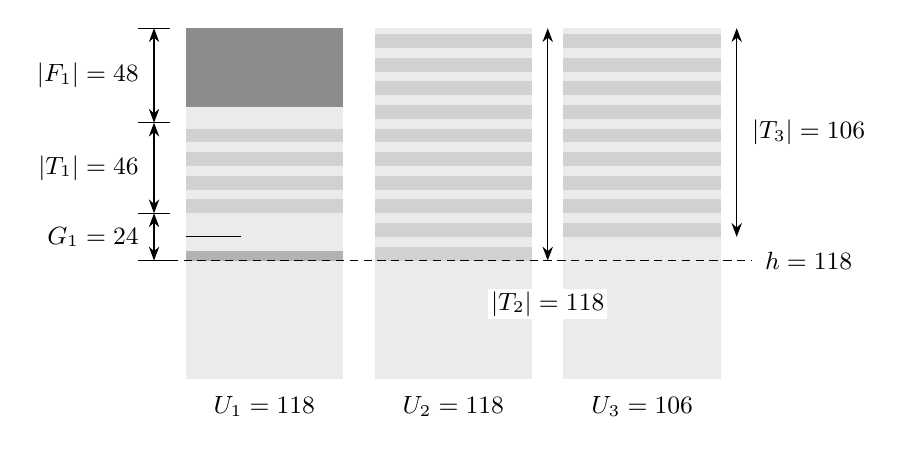
\begin{tikzpicture}[alg,x=1mm,y=-.25mm]
    \foreach \x in {0,24,48} {\excol{\x}{0}}
    \exfloat{0}{0}\exlines{0}{58}{4}\exfoot{0}{118}
    \exlines{24}{10}{10}
    \exlines{48}{10}{9}
    \draw[densely dashed] (-2,118) -- (72,118) node[right=1pt] {$h=118$};
    \draw[<->] (-4,0) -- (-4,48) node[midway,left=2pt] {$|F_1|=48$};
    \draw[<->] (-4,48) -- (-4,94) node[midway,left=2pt] {$|T_1|=46$};
    \draw[<->] (-4,94) -- (-4,118) node[midway,left=2pt] {$G_1=24$};
    \draw (-6,0) -- (-2,0) (-6,48) -- (-2,48) (-6,94) -- (-2,94) (-6,118) -- (-2,118);
    \draw[<->] (46,0) -- (46,118);
    \node[fill=white,inner sep=1pt] at (46,140) {$|T_2|=118$};
    \draw[<->] (70,0) -- (70,106) node[midway,right=2pt] {$|T_3|=106$};
    \foreach \x/\u in {10/{U_1=118},34/{U_2=118},58/{U_3=106}} {\node at (\x,192) {$\u$};}
  \end{tikzpicture}
  \caption{例\ref{ex:used}の所要の高さ（単位はpt）}
  \label{fig:ex-used}
\end{zu}

\begin{stmt}[見かけの下端]{定義}\label{def:bottom}
$d$を，$T$の行の深さのうち最も多い値とする（本文の行の標準の深さ）．配置の段$i$の
\kyocho{見かけの下端}$v_i$を，段の最後の要素に応じて次のように定める
（図\ref{fig:formal-even}）．
\begin{itemize}
  \item 本文の行で終わる段：最終行のベースラインの位置に$d$を足した位置．
  \item 下のフロートで終わる段：そのフロートの下端．
  \item 段の脚注で終わる段（\opt{footnote=column}）：脚注の最終行のベースラインを，本文の
    後で脚注が収まる最初の行の位置（$\tau+\ell b$の形の位置）に置いたときの，その位置に
    $d$を足した位置．
  \item 垂直の箱で終わり，中身が箱の下端より下に出ている段：中身の下端．
\end{itemize}
$v_i$を，段の最後の要素の基準線の位置$n_i$と，その下に見える分$e_i$の和$v_i=n_i+e_i$に
分けて書く．本文の行や段の脚注で終わる段では$e_i=d$，下のフロートで終わる段では
$e_i=0$である．
\end{stmt}

\begin{multicols}{2}
\begin{stmt}[見かけの下端]{例}\label{ex:bottom}
例\ref{ex:layout}の揃えた配置の見かけの下端を求める（図\ref{fig:ex-bottom}）．
\begin{itemize}
  \item 段2は本文の行で終わる．最終行のベースラインは$118$にあり，$v_2=118+d=121$．
  \item 段3も本文の行で終わる．最終行のベースラインは$106$にあり，$v_3=106+3=109$．
  \item 段1は段の脚注で終わる．本文の最終行のベースラインは$48+46=94$にある．その下に，
    行の深さ$3$と脚注の塊$20$の計$23$が要るので，脚注が収まる最初の行の位置は，2行下の
    $94+2\cdot12=118$である．脚注の最終行のベースラインをここに置くので，
    $v_1=118+3=121$．
\end{itemize}
（単位はpt．）定義\ref{def:bottom}の終わりの分け方では，$(n_1,n_2,n_3)=(118,118,106)$，
$e_i=3$である．
\end{stmt}
\end{multicols}

図\ref{fig:ex-bottom}の実線は最後の行のベースライン，破線は見かけの下端で，その差が
行の深さ$d=3\,\mathrm{pt}$である．段1の脚注は，本文の2行下の行の位置に最終行の
ベースラインを置く．

\begin{zu}
  \begin{tikzpicture}[alg,x=1mm,y=-.25mm]
    \foreach \x in {0,24,48} {\excol{\x}{0}}
    \exfloat{0}{0}\exlines{0}{58}{4}\exfoot{0}{118}
    \exlines{24}{10}{10}
    \exlines{48}{10}{9}
    \draw (-2,118) -- (44,118);
    \node[left=2pt] at (-2,112) {ベースライン$118$};
    \draw[densely dashed] (-2,121) -- (44,121);
    \node[left=2pt] at (-2,128) {$v_1=v_2=121$};
    \draw (48,106) -- (70,106) node[right=2pt,yshift=5pt] {ベースライン$106$};
    \draw[densely dashed] (48,109) -- (70,109) node[right=2pt,yshift=-5pt] {$v_3=109$};
  \end{tikzpicture}
  \caption{例\ref{ex:bottom}の見かけの下端（単位はpt）}
  \label{fig:ex-bottom}
\end{zu}

\section{釣り合いと整列：揃った配置と問題}\label{sec:f-even}

釣り合い（M5）と整列（M6）を，1つの定義にまとめる．条件の1と2が釣り合いで，途中の段を
1つの下端に合わせ，最後の段だけを短くてよいとする．条件の3が整列で，本文だけの段の
行を行の位置から動かさないことを求める．条件の3があるので，本文だけの段の行間を伸ばして
下端を合わせた配置は，揃った配置とは呼ばない．

\begin{stmt}[揃った配置]{定義}\label{def:even}
配置の中身のある最後の段を$L$とする（$L$より後の段は空）．配置が\kyocho{下端$\beta$で
揃っている}とは，次の3つが成り立つことをいう．
\begin{enumerate}
  \item $i<L$のすべての段で，グルーを伸び縮みさせて$v_i=\beta$にできる．
  \item $v_L\le\beta$（最後の段は短くてよいが，高くはしない）．
  \item 本文だけの段（フロートも脚注もない段）では，グルーを伸び縮みさせない．つまり，
    行の位置は，\LaTeX{}が組むときの位置のままである．
\end{enumerate}
\end{stmt}

図\ref{fig:formal-even}の帯は行で，帯の下辺がベースラインである．段1は本文だけの段で，
行は$\tau+\ell b$の位置から動かさない．段2は，本文と下のフロートの間のアキを伸び縮み
させて，フロートの下端を$\beta$に合わせる．段3は中身のある最後の段$L$で，$\beta$より
高くなければよい．段の脚注の最終行は，行の位置（$\tau+\ell b$）に置く．{\widowpenalty=10000\par}

\begin{figure}[tbp]
  \centering
  \begin{tikzpicture}[alg,x=.9mm,y=.9mm,
      txt/.style={fill=black!18},fl/.style={fill=black!45}]
    %% 段1：本文だけ
    \foreach \i in {0,...,11} \fill[txt] (0,59.2-4*\i) rectangle (30,57-4*\i);
    \draw[|-|] (-3,60) -- node[lab,left=4pt] {$\tau$} (-3,57);
    \draw[|-|] (-3,53) -- node[lab,left=4pt] {$b$} (-3,49);
    \node[lab,above] at (15,60) {段1};
    %% 段2：下のフロート
    \foreach \i in {0,...,6} \fill[txt] (48,59.2-4*\i) rectangle (78,57-4*\i);
    \fill[fl] (48,12) rectangle (78,25);
    \node[lab,text=white] at (63,18.5) {下のフロート};
    \draw[|-|] (45,32) -- node[lab,left] {アキ} (45,25);
    \node[lab,above] at (63,60) {段2};
    %% 段3：脚注で終わる最後の段
    \foreach \i in {0,...,5} \fill[txt] (96,59.2-4*\i) rectangle (126,57-4*\i);
    \draw (96,32.5) -- (106,32.5);
    \fill[txt] (96,28.8) rectangle (126,30.4);
    \fill[txt] (96,25) rectangle (114,26.6);
    \node[lab,above] at (111,60) {段3（$=L$）};
    \draw[densely dashed] (93,24) -- (129,24);
    \node[lab,right] at (129,24) {$v_3$};
    %% 下端
    \draw[densely dashed] (-6,12) -- (129,12);
    \node[lab,right] at (129,12) {$\beta$};
    \node[lab,below,align=center] at (15,10) {本文の行で終わる段\\$v_1=$最終行のベースライン$+d$};
    \node[lab,below,align=center] at (63,10) {下のフロートで終わる段\\$v_2=$フロートの下端};
    \node[lab,below,align=center] at (111,10) {脚注で終わる段\\$v_3\le\beta$（最後の段は短くてよい）};
  \end{tikzpicture}
  \caption{見かけの下端と揃った配置（定義\ref{def:bottom}，\ref{def:even}）}
  \label{fig:formal-even}
  \setteizu{\texttt{\cs{begin}\{figure\}[tbp]}}
\end{figure}

\begin{multicols}{2}
\begin{stmt}[揃った配置]{例}\label{ex:even}
例\ref{ex:bottom}の配置は，下端$\beta=121\,\mathrm{pt}$で揃っている（図\ref{fig:ex-even}の左）．
中身のある最後の段は$L=3$である．
\begin{enumerate}
  \item 段1と段2は$v_1=v_2=121=\beta$で，グルーを伸び縮みさせるまでもない．
  \item $v_3=109\le\beta$．
  \item 本文だけの段2と段3は，行の位置を動かしていない．
\end{enumerate}
揃っていない配置の例として，同じ材料で切れ目を$k'=(0,4,13,23)$とする
（図\ref{fig:ex-even}の右）．段2が9行，段3が10行で，見かけの下端は
$(v_1,v_2,v_3)=(121,109,121)$になる．段2は本文だけの段なので，3から伸ばせず，1を満たすには
$\beta=109$とするしかない．しかし$v_3=121>109$で，2に反する．よって，この配置は，
どの$\beta$でも揃っていない．
\end{stmt}
\settei{\texttt{\cs{begin}\{multicols\}\{2\}}}
\end{multicols}

図\ref{fig:ex-even}の左は，下端$\beta$で揃った配置である．最後の段3は短くてよい．右は，
途中の段2が1行分短い配置である．段2は本文だけの段で伸ばせないので，揃っていない
（どちらも，段の下の部分は省いてある）．

\begin{zu}
  \begin{tikzpicture}[alg,x=1mm,y=-.25mm]
    \foreach \x in {0,24,48} {\excol[136]{\x}{0}}
    \exfloat{0}{0}\exlines{0}{58}{4}\exfoot{0}{118}
    \exlines{24}{10}{10}
    \exlines{48}{10}{9}
    \draw[densely dashed] (-2,121) -- (70,121) node[right=1pt] {$\beta$};
    \node at (34,150) {$k=(0,4,14,23)$：揃っている};
    \begin{scope}[xshift=78mm]
      \foreach \x in {0,24,48} {\excol[136]{\x}{0}}
      \exfloat{0}{0}\exlines{0}{58}{4}\exfoot{0}{118}
      \exlines{24}{10}{9}
      \exlines{48}{10}{10}
      \draw[densely dashed] (-2,121) -- (70,121);
      \draw[<->] (34,109) -- (34,121);
      \node[right=1pt,font=\footnotesize] at (34,128) {1行分短い};
      \node at (34,150) {$k'=(0,4,13,23)$：揃っていない};
    \end{scope}
  \end{tikzpicture}
  \caption{例\ref{ex:even}の2つの配置}
  \label{fig:ex-even}
\end{zu}

\par\addvspace{.5\baselineskip}
\noindent\begin{minipage}{\linewidth}
\komidashi{問題}
ここまでの定義で，要請を問題の条件に置き換える．
\begin{tcolorbox}
\begin{stmt}[最終ページを揃える]{問題}\label{prob:main}
材料$M$，段数$N$，段の高さ$H$が与えられ，$M$は\LaTeX{}が高さ$H$の$N$段に組んだものと
する．次を満たす配置$(k,s)$と高さ$h\le H$を求めよ．
\begin{multicols}{2}
\begin{enumerate}
  \item[(P1)\hspace{.5\zw}] 配置は$h$に入り切る．
  \item[(P2)\hspace{.5\zw}] 順序を保つ．本文は読む順のまま（切れ目$k$で分けるだけ），フロートは
    $s\in S$．
  \item[(P3)\hspace{.5\zw}] 脚注は，\opt{footnote=column}では参照位置と同じ段の下端に，
    \opt{footnote=page}では版面の下端に全幅で置く．
  \item[(P4)\hspace{.5\zw}] 配置は，ある下端$\beta\le h$で揃っている．
  \item[(P5)\hspace{.5\zw}] (P1)から(P4)を満たすもののうちで，$h$が最も小さい．$h$の差が1行未満なら，
    動かすフロートの少ないものを選ぶ．動かす量は$\mu(s)=\sum_j(s(j)-o_j)$で測る．
\end{enumerate}
\end{multicols}
\end{stmt}
\settei[この箱の設定]{\texttt{tcolorbox}の中に\texttt{\cs{begin}\{multicols\}\{2\}}}
\end{tcolorbox}
\end{minipage}
\par\addvspace{.5\baselineskip}

\begin{evenendmulticols}[columnsep=3\zw,columnseprule=.4pt]{2}
\begin{stmt}{注意}\label{rem:exist}
行もフロートも分けられないので，(P4)を満たす配置があるとは限らない．また，(P1)は
\LaTeX{}の配置$(k^0,s^0)$が$h=H$で満たすように見えるが，定義\ref{def:used}の切り上げの
分だけ所要の高さが増えるので，これも保証されない．そこで実装は，問題\ref{prob:main}の
厳密な解ではなく，次の節の手順が与える配置を解とする．解が得られない場合の扱いも，
手順の中で定める．手順について証明できることと，証明しないことは，命題\ref{prop:main}と
注意\ref{rem:noproof}に分けて述べる．
\end{stmt}
\settei{\texttt{\cs{begin}\{evenendmulticols\}[columnsep=3\cs{zw},\allowbreak columnseprule=.4pt]\{2\}}}
\end{evenendmulticols}

\komidashi{要請と条件の対応}
\begin{multicols}{2}
問題\ref{prob:main}の条件は，要請に次のように対応する．
\begin{itemize}
  \item (P1)は版面（M2）．段の高さ$H$を超えない．
  \item (P2)は読む順序（M3）．
  \item (P3)は配置（M4）のうち，脚注の置き場所．図表の置き場所（上のフロートは段の上端，
    下のフロートは段の下端）は，段を組む手順（命題\ref{prop:main}の手順5）で定める．
  \item (P4)は釣り合い（M5）と整列（M6）．
  \item (P5)の前半は余白（M7）．$h$を最も小さくすれば，段組の下の余白が最も大きくなる．
    後半は一貫性（M8）で，図表をなるべく動かさない．
\end{itemize}
構造（M1）は，条件としては現れない．$N$，$b$，$\tau$を与えられたものとして変えない
ことが，それにあたる．(P1)から(P4)は満たすべき条件，(P5)は条件を満たすものの中での
選び方である．つまり，版面，読む順序，配置，釣り合いと整列を先に守り，余白と一貫性は
その中で選ぶ．
\end{multicols}

\section{手順と証明}\label{sec:f-proc}

手順は，3つの層からなる．割り振りと高さを決めて本文を段に分ける貪欲な分割
（補題\ref{lem:fill}），割り振りごとに段組の最も低い高さを探す手順（補題\ref{lem:minh}），
候補を選んで段を組む全体の手順（命題\ref{prop:main}）である．版面，読む順序，脚注の
置き場所（M2からM4）は，最も内側の貪欲な分割が守る．余白（M7）は高さを探す層が，
一貫性（M8）と釣り合い（M5），整列（M6）は全体の手順が受け持つ．

割り振り$s$と高さ$h$を決めれば，切れ目は貪欲に決まる．

\begin{stmt}[貪欲な分割]{補題}\label{lem:fill}
$s\in S$と$h\le H$に対し，次の手順$\mathrm{Fill}(s,h)$は，高々$10(N-1)$回の
\cs{vsplit}で止まり，配置$(k,s)$を1つ返すか，失敗する．返した配置は(P1)から(P3)を
満たす．
\end{stmt}
\begin{tejun}
$i=1,\dots,N-1$の順に，残りの本文の先頭から段$i$の本文を切り出す
（図\ref{fig:formal-fill}）．
\begin{enumerate}
  \item 本文に使える高さを$c=h-|F_i|-G$とする．初めは，$G$を，段$i$に必ず入る脚注
    だけの高さとする．$c<0$なら失敗とする．
  \item 残りの本文から，\TeX{}の\cs{vsplit}で高さ$c$までを切り出す．\cs{vsplit}は，$c$を
    超えない最もよい切れ目を選ぶ．これを$T_i$とする．
  \item $T_i$に参照位置のある脚注から$G_i$を求め直す．$|F_i|+|T_i|+G_i\le h$なら，この段を
    確定する．
  \item 超えていれば，超えた分だけ$c$を小さくして，2からやり直す．10回くり返しても
    収まらなければ失敗とする．
\end{enumerate}
最後に，残りの本文のすべてを$T_N$とする．$U_N\le h$で，$T_N$に強制の改段が残って
いなければ，配置を返す．そうでなければ失敗とする．
\end{tejun}
\begin{multicols}{2}
\begin{shoumei}
\kyocho{止まること}．段$1$から$N-1$のそれぞれで，2から4のくり返しは高々10回である．
1回のくり返しで\cs{vsplit}を1回使うので，\cs{vsplit}は高々$10(N-1)$回である．

\kyocho{(P1)}．$i<N$の段は，3で$|F_i|+|T_i|+G_i\le h$を確かめたときにだけ確定する．
段$N$は，最後に$U_N\le h$を確かめる．$|F_i|$は$s$だけで決まる．後の段の切り出しは残りの
本文だけを使うので，確定した段の$T_i$は変わらず，$|T_i|$と$G_i$も変わらない．
したがって，返した配置ではすべての段で$U_i\le h$である．

\kyocho{(P2)}．\cs{vsplit}は，残りの本文の先頭から，改ページできる位置までを，要素の順を
変えずに切り出す．このとき，切れ目から残りの最初の箱までにある捨てられる要素（グルー，
カーン，ペナルティ）を捨てる．その間にある捨てられない要素（\cs{special}や\cs{mark}の
印など）は残す．残りの先頭には，\cs{splittopskip}のグルーが1つ入る．つまり，捨てられる
要素のほかは，何も失われず，順も変わらない．段の先頭に来た捨てられる要素を除くのは，
定義\ref{def:layout}のとおりである．よって，切り出した$T_1,\dots,T_N$は，ある切れ目
$k_0\le\dots\le k_N$による分割で，本文は読む順のままである．$s$は，初めから$S$の
元である．

\kyocho{(P3)}．3の$G_i$は，参照位置が$T_i$に入る脚注の集合$\Phi_i$だけから求める．
参照位置は，行の直後に置いた印（番号を持つ）でわかる．\opt{footnote=column}では，
(P1)から，どの段も本文の下に$\Phi_i$を積む高さ$G_i$を$h$の中に持つ．よって，脚注を
参照位置と同じ段の下端に置ける．\opt{footnote=page}では，$H$からページの脚注の領域を
引いてある（定義\ref{def:used}）．$h\le H$なので，どの段もその領域に掛からず，脚注を
版面の下端に全幅で置ける．
\end{shoumei}
\settei{\texttt{\cs{begin}\{multicols\}\{2\}}}
\end{multicols}

図\ref{fig:formal-fill}に，段$i$の切り出しを示す．初めは，脚注を見込まずに高さ$c$まで
本文を切り出す．切り出した本文に脚注の参照（\textdagger）があると，脚注の分だけ$h$を
超える．超えた分だけ$c$を小さくして切り直し，$|F_i|+|T_i|+G_i\le h$になれば段を確定する．
切り出さなかった行は，次の段へ回る．

\begin{figure}[tbp]
  \centering
  \begin{tikzpicture}[alg,x=.9mm,y=.9mm,
      txt/.style={fill=black!18},fl/.style={fill=black!45}]
    \draw[densely dashed] (-8,0) -- (136,0);
    \draw[<->] (-5,0) -- node[lab,left] {$h$} (-5,50);
    %% 手順1，2
    \fill[fl] (0,42) rectangle (28,50);
    \node[lab,text=white] at (14,46) {フロート};
    \foreach \i in {0,...,9} \fill[txt] (0,40.8-4*\i) rectangle (28,38.6-4*\i);
    \node[lab] at (29.6,17.2) {\textdagger};
    \draw[|-|] (34,50) -- node[lab,right] {$|F_i|$} (34,42);
    \draw[|-|] (34,42) -- node[lab,right] {$c$} (34,0);
    \node[lab,below,align=center] at (14,-11) {手順1，2：$c=h-|F_i|-G$\\まで\cs{vsplit}で切り出す};
    \draw[->] (41,25) -- (49,25);
    %% 手順3
    \begin{scope}[xshift=46.8mm]
      \fill[fl] (0,42) rectangle (28,50);
      \foreach \i in {0,...,9} \fill[txt] (0,40.8-4*\i) rectangle (28,38.6-4*\i);
      \node[lab] at (29.6,17.2) {\textdagger};
      \draw (0,-2) -- (9,-2);
      \fill[txt] (0,-5.6) rectangle (28,-4);
      \fill[txt] (0,-9) rectangle (16,-7.4);
      \draw[|-|] (31,-0.3) -- (31,-9);
      \node[lab,right] at (32,-5.5) {超えた分};
      \node[lab,right] at (16.5,-8.2) {脚注};
      \node[lab,below,align=center] at (14,-11) {手順3：脚注を求め直すと\\$h$を超える};
    \end{scope}
    \draw[->] (93,25) -- (101,25);
    %% 手順4
    \begin{scope}[xshift=93.6mm]
      \fill[fl] (0,42) rectangle (28,50);
      \foreach \i in {0,...,6} \fill[txt] (0,40.8-4*\i) rectangle (28,38.6-4*\i);
      \node[lab] at (29.6,17.2) {\textdagger};
      \draw (0,9) -- (9,9);
      \fill[txt] (0,5.4) rectangle (28,7);
      \fill[txt] (0,2) rectangle (16,3.6);
      \draw[|-|] (34,42) -- node[lab,right] {$c'$} (34,12);
      \draw[|-|] (34,12) -- node[lab,right] {$G_i$} (34,0);
      \node[lab,below,align=center] at (14,-11) {手順4：$c$を小さくして\\切り直すと入り切る};
    \end{scope}
  \end{tikzpicture}
  \caption{貪欲な分割$\mathrm{Fill}$の段$i$の切り出し（補題\ref{lem:fill}）}
  \label{fig:formal-fill}
  \setteizu{\texttt{\cs{begin}\{figure\}[tbp]}}
\end{figure}

\begin{stmt}{注意}
$\mathrm{Fill}$は貪欲で，前の段にできるだけ多く入れる．$h$に入り切る配置があっても，
$\mathrm{Fill}(s,h)$が失敗することはありうる．また，$\mathrm{Fill}(s,h)$が成功
するかどうかは，$h$について単調とは限らない．切れ目が変わると，脚注の入る段が変わる
ためである．
\end{stmt}

\begin{stmt}[割り振りごとの最小の高さ]{補題}\label{lem:minh}
$s\in S$に対し，次の手順は，高々
$\max\{0,\lceil\log_2((H-h_0)/1\,\mathrm{pt})\rceil\}+6$回の$\mathrm{Fill}$で止まり，
$\mathrm{Fill}(s,h)$が成功する高さ$h(s)\le H$を1つ返すか，「入り切らない」と
答える．$h_0$は，手順の中で定める下界である．{\widowpenalty=10000\par}
\end{stmt}
\begin{tejun}
$\mathrm{Fill}(s,H)$が失敗すれば，「入り切らない」と答える．成功すれば，下界を
\[ h_0=\Bigl\lfloor\bigl(|T|+\textstyle\sum_j|f_j|\bigr)/N\Bigr\rfloor-2b \]
とし，区間$[h_0,H]$を二分法で狭める（図\ref{fig:formal-minh}）．中点で$\mathrm{Fill}$が成功すれば上端を，失敗すれば
下端を中点に移し，幅が1ptになるまで続ける．上端を$h_1$とする．$\mathrm{Fill}$の成否は
単調とは限らないので，最後に$h_1-4\,\mathrm{pt}$から$h_1$まで1ptずつ調べ，最初に成功した
高さを$h(s)$とする．ただし，下界$h_0$より下は調べない（$h_1-4\,\mathrm{pt}$が$h_0$より
下になるときは，$h_0$から調べる）．$h_0$が負になるときは，$h_0=0$とする．{\widowpenalty=10000\par}
\end{tejun}
\begin{shoumei}
二分法のあいだ，区間の上端では，つねに$\mathrm{Fill}$が成功する．初めの上端$H$では
$\mathrm{Fill}(s,H)$が成功しており，上端を移すのは，中点で成功したときだけだからで
ある．よって，$h_1$で$\mathrm{Fill}$は成功する．最後の調べ直しは$h_1$で終わるので
（調べる範囲が空のときは$h_1$を返す），成功する高さが必ずあり，$h(s)\le h_1\le H$で
ある．

$\mathrm{Fill}$の回数は，初めの1回，二分法の
$\max\{0,\lceil\log_2((H-h_0)/1\,\mathrm{pt})\rceil\}$回（1回ごとに区間の幅が半分になる），
調べ直しの高々5回である．
\end{shoumei}

\begin{stmt}{注意}\label{rem:minh}
$h(s)$は，$\mathrm{Fill}(s,h)$が成功する最小の$h$とは限らない．成否が単調で
ないので，二分法が捨てた区間（失敗した中点より下）に，成功する高さが残りうる．
補題\ref{lem:minh}から言えるのは，$h(s)$で成功することと，調べ直した高さのうち
$h(s)$より低いものでは失敗することだけである．
\end{stmt}

図\ref{fig:formal-minh}の上では，区間$[h_0,H]$を二分法で狭めている．数字は調べる順
（3回目まで），○は$\mathrm{Fill}$の成功，×は失敗で，太線は成功する範囲である．幅が
1ptになったときの上端を$h_1$とする．成否は単調とは限らないので，図の下のように，$h_1$の
4pt下から1ptずつ調べ，最初に成功した高さを$h(s)$とする．

\begin{figure}[tbp]
  \centering
  \begin{tikzpicture}[alg,x=.9mm,y=.9mm]
    %% 二分法
    \node[lab,left] at (-6,30) {二分法};
    \draw (0,30) -- (120,30);
    \draw[line width=3pt,black!45] (82,30) -- (120,30);
    \draw (0,28) -- (0,32) node[lab,above] {$h_0$};
    \draw (120,28) -- (120,32) node[lab,above] {$H$};
    \foreach \x/\n/\m in {60/1/×,90/2/○,75/3/×}
      {\draw (\x,28.5) -- (\x,31.5);
       \node[lab,above] at (\x,32) {\m};
       \node[lab,above] at (\x,36) {\n};}
    \draw (82,27) -- (82,33) node[lab,above] {$h_1$};
    \node[lab,below] at (30,28) {失敗する};
    \node[lab,below] at (104,28) {成功する};
    %% 下から調べ直す
    \draw[densely dotted] (82,26.5) -- (16,12) (82,26.5) -- (84,12);
    \node[lab,left,align=right] at (-6,6) {下から\\調べ直す};
    \draw (10,6) -- (90,6);
    \foreach \x/\t/\m in {20/{$h_1-4$}/×,35/{$h_1-3$}/○,50/{$h_1-2$}/×,65/{$h_1-1$}/×,80/{$h_1$}/○}
      {\draw (\x,4.5) -- (\x,7.5);
       \node[lab,above] at (\x,8) {\m};
       \node[lab,below] at (\x,4) {\t};}
    \node[lab,right] at (91,6) {（pt）};
    \draw[->] (35,-7) -- (35,-1.5);
    \node[lab,below] at (35,-7) {$h(s)$：最初に成功した高さ};
  \end{tikzpicture}
  \caption{割り振りごとの最小の高さの探し方（補題\ref{lem:minh}）}
  \label{fig:formal-minh}
  \setteizu{\texttt{\cs{begin}\{figure\}[tbp]}}
\end{figure}

\begin{stmt}[揃えた配置の構成]{命題}\label{prop:main}
次の手順は，有限回の$\mathrm{Fill}$で止まり，配置$(k,s)$と下端$\beta$を返すか，
「揃えられない」と答える．返した配置と$\beta$について，次が成り立つ．
\begin{enumerate}
  \item[(i)\hspace{.5\zw}] ある$h\le H$について，配置は(P1)から(P3)を満たす．
  \item[(ii)\hspace{.5\zw}] どの段の見かけの下端も，フロートまわりのグルーの縮みの範囲で
    $\beta$以下にできる．とくに，定義\ref{def:even}の2（$v_L\le\beta$）にあたる条件が
    成り立つ．
\end{enumerate}
定義\ref{def:even}の1（途中の段を$\beta$に合わせられること）は，命題\ref{prop:even}で
条件を付けて示す．(P4)の残りと(P5)は主張しない（注意\ref{rem:noproof}）．
\end{stmt}
\begin{tejun}
\begin{enumerate}
  \item \kyocho{候補を挙げる}．$S$の割り振りを列挙する．64個を超えるときは，\LaTeX{}が
    置いたフロートを動かさず（$s(j)=o_j$），持ち越したフロートだけを動かす候補に限る．
    段をまたぐフロートが同じ位置で同じ段に重なる候補は除く．{\widowpenalty=10000\par}
  \item \kyocho{高さを求める}．各候補$s$について，補題\ref{lem:minh}で$h(s)$を
    求める．
  \item \kyocho{候補を選ぶ}．候補を順に見て，それまでの最良$(s^*,h^*)$を次の規則で
    置き換える．$\mu(s)<\mu(s^*)$のときは，$h(s)<h^*+b$なら置き換える（動かす
    フロートが少なければ，1行未満の高さの差は許す）．$\mu(s)=\mu(s^*)$のときは，
    $h(s)<h^*$なら置き換える．$\mu(s)>\mu(s^*)$のときは，
    $h(s)\le h^*-b$のときだけ置き換える（フロートを余計に動かすのは，1行以上低く
    なるときだけ）．高さの比較には，高さを調べる刻み（1pt）の半分の余裕を持たせる．
    どの候補も入り切らなければ，手順6へ進む．
  \item \kyocho{揃わない配分を直す}．$\mathrm{Fill}(s^*,h^*)$の配置の$v_1,\dots,v_N$を
    測る．次のどれかが成り立てば，揃わない配分とみなす
    （図\ref{fig:formal-misaligned}）．
    \begin{enumerate}
      \item $v_N>\max_{i<N}v_i$（最右段がほかのどの段よりも高い）．
      \item 本文だけの段の見かけの下端の最大を$\beta_T$として，後ろに中身のある途中の段で
        $v_i<\beta_T-b/2$（途中の段が明らかに短い）．
      \item フロートまわりのグルーを縮めても，$v_i>\beta_T$となる段がある．
    \end{enumerate}
    揃わない配分なら，$h$を$h^*$から1ptずつ上げて$\mathrm{Fill}(s^*,h)$をやり直し，
    揃わない配分でなくなった最初の$h$を採る．$H$まで上げても見つからなければ，元の配置の
    ままとする．
  \item \kyocho{段を組む}．$\beta=\max_i v_i$とする．本文だけの段があり，ほかの段を
    グルーの縮みで$\beta_T$に合わせられるなら，$\beta=\beta_T$とする（本文だけの段を基準に
    する）．各段を，上のフロート，本文，下のフロート，脚注の順に積み，
    高さ$\beta-e_i$の箱に組む（定義\ref{def:bottom}の$e_i$）．このとき，次の所に，無限に
    伸びるグルーを入れる．
    \begin{enumerate}
      \item 段の脚注のある段：本文の後（下のフロートがあれば，その前）．脚注と下の
        フロートを箱の下端に付ける．
      \item 下のフロートのある段で，段のグルーの伸びの和が不足$\beta-v_i$に足りない
        とき：本文と下のフロートの間（フロートを箱の下端に付ける）．
      \item 段$L$と，次の段に中身のある途中の段で，不足$\beta-v_i$が半行（$b/2$）を
        超えるとき：本文の末尾（行を動かさずに下を空ける）．
    \end{enumerate}
    ほかのグルーは，\TeX{}が箱の高さに合わせて伸び縮みさせる．配置と$\beta$を返す
    （実装は，$\beta$を揃えた段組の高さとして使う）．
  \item \kyocho{緩める}．どの候補も入り切らないときは，条件を1つ緩めて，手順1から
    やり直す．1回目は，脚注の塊を$b$の倍数に切り上げない（定義\ref{def:used}）．2回目は，
    \opt{floatgrid}もやめる．それでも入り切らなければ，「揃えられない」と答える．このとき
    \TeX{}側は，\LaTeX{}の配置$(k^0,s^0)$のままページを出力し，警告を出す．
\end{enumerate}
\end{tejun}
%% 調整：図12は，初めに参照する手順4の近くに出るように，手順の後に置いてある
\begin{figure}[tbp]
  \centering
  \begin{tikzpicture}[alg,x=.9mm,y=.9mm,
      txt/.style={fill=black!18},fl/.style={fill=black!45}]
    %% (a)
    \begin{scope}
      \foreach \i in {0,...,4} {\fill[txt] (0,30-3*\i) rectangle (8,28.2-3*\i);
        \fill[txt] (10,30-3*\i) rectangle (18,28.2-3*\i);}
      \foreach \i in {0,...,6} \fill[txt] (20,30-3*\i) rectangle (28,28.2-3*\i);
      \draw[densely dashed] (-2,15.6) -- (30,15.6);
      \node[lab,below,align=center] at (14,7) {(a) 最右段がどの段\\よりも高い};
    \end{scope}
    %% (b)
    \begin{scope}[xshift=32.4mm]
      \foreach \i in {0,...,6} \fill[txt] (0,30-3*\i) rectangle (8,28.2-3*\i);
      \foreach \i in {0,...,4} \fill[txt] (10,30-3*\i) rectangle (18,28.2-3*\i);
      \foreach \i in {0,...,5} \fill[txt] (20,30-3*\i) rectangle (28,28.2-3*\i);
      \draw[densely dashed] (-2,9.6) -- (30,9.6);
      \draw[|-|] (14,15.6) -- (14,9.6);
      \node[lab,below,align=center] at (14,7) {(b) 途中の段が\\半行以上短い};
    \end{scope}
    %% (c)
    \begin{scope}[xshift=64.8mm]
      \foreach \i in {0,...,6} \fill[txt] (0,30-3*\i) rectangle (8,28.2-3*\i);
      \fill[fl] (10,22) rectangle (18,30);
      \foreach \i in {0,...,4} \fill[txt] (10,20.5-3*\i) rectangle (18,18.7-3*\i);
      \foreach \i in {0,...,5} \fill[txt] (20,30-3*\i) rectangle (28,28.2-3*\i);
      \draw[densely dashed] (-2,9.6) -- (30,9.6);
      \node[lab,below,align=center] at (14,7) {(c) 縮めても$\beta_T$を\\超える};
    \end{scope}
    \draw[->] (106,17) -- (124,17);
    \node[lab,align=center,anchor=south] at (115,20) {$h$を1ptずつ\\上げて\\分け直す};
    %% 揃う配分
    \begin{scope}[xshift=115.2mm]
      \foreach \i in {0,...,6} {\fill[txt] (0,30-3*\i) rectangle (8,28.2-3*\i);
        \fill[txt] (10,30-3*\i) rectangle (18,28.2-3*\i);}
      \foreach \i in {0,...,4} \fill[txt] (20,30-3*\i) rectangle (28,28.2-3*\i);
      \draw[densely dashed] (-2,9.6) -- (30,9.6);
      \node[lab,below,align=center] at (14,7) {判定を通る配分};
    \end{scope}
  \end{tikzpicture}
  \caption{揃わない配分（命題\ref{prop:main}の手順4）}
  \label{fig:formal-misaligned}
  \setteizu{\texttt{\cs{begin}\{figure\}[tbp]}}
\end{figure}
\begin{multicols}{2}
\begin{shoumei}
\kyocho{止まること}．手順1の候補は高々257個である．手順2は，候補ごとに
補題\ref{lem:minh}の回数の$\mathrm{Fill}$で終わる．手順4は，$h$を1ptずつ$H$まで上げる
だけなので，高々$(H-h^*)/1\,\mathrm{pt}$回の$\mathrm{Fill}$で終わる．手順3と5は
$\mathrm{Fill}$を使わない．手順6から手順1へ戻るのは高々2回なので，全体は高々3巡で
終わる．$\mathrm{Fill}$そのものは，補題\ref{lem:fill}から，高々$10(N-1)$回の\cs{vsplit}で
止まる．

\kyocho{(i)}．配置を返すのは，手順3で候補が選ばれたときだけである．このとき返す配置は，
$\mathrm{Fill}(s^*,h^*)$が返したものか，手順4の$\mathrm{Fill}(s^*,h)$
（$h^*<h\le H$）が返したものである．$h^*=h(s^*)\le H$は，補題\ref{lem:minh}による．
手順5は，切れ目も割り振りも変えない．よって，補題\ref{lem:fill}から，配置はその$h$に
ついて(P1)から(P3)を満たす．手順6で条件を緩めた後は，緩めた$G_i$で定めた所要の高さに
ついて同じことが成り立つ．

\kyocho{(ii)}．手順5で$\beta=\max_i v_i$としたときは，すべての段で$v_i\le\beta$である．
$\beta=\beta_T$とするのは，すべての段で，$v_i$からフロートまわりのグルーの縮みを引いた
値が$\beta_T$以下のときだけである．どちらの場合も，主張が成り立つ．
\end{shoumei}
\end{multicols}

\komidashi{手順と要請の対応}
\begin{multicols}{2}
命題\ref{prop:main}の手順のそれぞれが，どの要請のためにあるかを記す．
\begin{itemize}
  \item 手順1から3は，余白（M7）と一貫性（M8）の折り合いである．段組が最も低くなる
    割り振りを探すが，図表を余計に動かすのは，1行以上低くなるときだけにする．
  \item 手順4は，釣り合い（M5）と整列（M6）の折り合いである．最も低い高さで分けた配置が
    揃わないとき，行間を伸ばすのではなく，高さを上げて分け直す．余白（M7）を譲って，
    行の位置を守る．
  \item 手順5は，整列（M6）と余白（M7）のうち，アキの入れ場所を定める．本文だけの段を
    基準にして下端を決め，伸び縮みは図表のまわりのグルーに持たせる．無限に伸びるグルーを
    入れる3つの場所は，どれも本文と脚注，本文と図表の境か，本文の末尾で，行間ではない．
  \item 手順6は，入り切らないときに譲る順を定める．まず脚注の高さの切り上げを，次に
    フロートの前後の行の位置合わせをやめる．版面（M2）を守るために，整列（M6）の一部を
    譲る．
\end{itemize}
\end{multicols}

\begin{stmt}[段が揃うための条件]{命題}\label{prop:even}
命題\ref{prop:main}の手順が返した配置と$\beta$について，次が成り立つ．
\begin{enumerate}
  \item[(i)\hspace{.5\zw}] $v_i>\beta$の段は，手順5でグルーが縮み，見かけの下端が$\beta$に
    なる．
  \item[(ii)\hspace{.5\zw}] $v_i<\beta$の段$i<L$は，次の3つを満たせば，手順5で見かけの
    下端が$\beta$になる．
    \begin{enumerate}
      \item 不足が半行以下である：$\beta-v_i\le b/2$．
      \item 段の並びが，最後の要素（行，下のフロート，脚注）で終わる．つまり，最後の
        要素の後ろにグルーがない．
      \item 段が，段の脚注か下のフロートで終わる．または，段のグルーの伸びの和が正で
        ある．
    \end{enumerate}
\end{enumerate}
したがって，$i<L$のすべての段が(ii)の3つを満たすか$v_i\ge\beta$であれば，
定義\ref{def:even}の1と2が成り立つ．\opt{footnote=page}では，段がページの脚注の領域に
掛からないことも仮定する．\cs{columnbreak}で終わる段は，最後の行の後ろに
\cs{vfil}が残るので，(b)を満たさない．
\end{stmt}
\begin{multicols}{2}
\begin{shoumei}
\TeX{}は，高さを指定して箱を組むとき，中身の自然な高さと指定の差を，グルーに割り振る．
自然な高さが指定より小さいとき，無限に伸びるグルーがあれば，そのグルーだけが差を
受け持つ．なければ，伸びの和が正である限り，有限の伸びに比例して差の全部を割り振る．
自然な高さが指定より大きいときは，縮みの和が差以上であれば，縮みに比例して差の全部を
割り振る．差の全部が割り振られ，それを受け持つグルーが最後の要素より上にあれば，
最後の要素の基準線は箱の下端に来る．

手順5は，段$i$を高さ$\beta-e_i$の箱に組む．最後の要素の基準線が箱の下端に来れば，
見かけの下端は$(\beta-e_i)+e_i=\beta$である．そこで，差の全部がグルーに割り振られ，
しかも最後の要素が動くことを，場合ごとに確かめる．

\kyocho{(i)}．$v_i>\beta$の段があるのは，手順5で$\beta=\beta_T$としたときだけである
（$\beta=\max_i v_i$なら，そのような段はない）．このとき手順5は，すべての段で，$v_i$から
フロートまわりのグルーの縮みを引いた値が$\beta_T$以下であることを確かめている．
フロートまわりのグルーの縮みは，段のグルーの縮みの和以下である．よって，縮みの和は
差$v_i-\beta$以上で，差の全部が割り振られる．

\kyocho{(ii)}．(a)から，手順5の3の無限に伸びるグルーは入らない．(b)から，段のグルーは
どれも最後の要素より上にある．(c)を3つに分ける．
段の脚注で終わる段では，手順5の1のグルーが無限に伸びるので，差の全部が無限に伸びる
グルーに割り振られ，脚注が箱の下端まで下がる．
下のフロートで終わる段では，伸びの和が不足に足りなければ，手順5の2のグルーが入り，
同じく差の全部が割り振られて，フロートが箱の下端まで下がる．足りていれば，伸びの和は
正なので，差の全部が割り振られる．
どちらでもない段では，伸びの和が正なので，差の全部が割り振られる．
どの場合も，差を受け持つグルーは最後の要素より上にあるので，最後の要素の基準線は
箱の下端に来る．

\kyocho{定義\ref{def:even}の1と2}．1は，(i)と(ii)と，$v_i=\beta$の段では差がないこと
による．2は，命題\ref{prop:main}の(ii)による．
\end{shoumei}
\end{multicols}

\begin{multicols}{2}
\begin{stmt}[証明しないこと]{注意}\label{rem:noproof}
命題\ref{prop:main}と命題\ref{prop:even}は，次の性質を主張しない．手順はこれらを目指して
作ってあるが，次のとおり，材料によっては成り立たない．
\begin{itemize}
  \item \kyocho{途中の段を$\beta$に合わせられること}（定義\ref{def:even}の1）．
    命題\ref{prop:even}の(ii)の条件を欠く段は，揃わない．不足が半行を超える段と，
    伸びるグルーのない本文だけの段は，行を動かさずに下が空く．最後の行の後ろに
    \cs{vfil}の残る段（\cs{columnbreak}で終わる段）は，\cs{vfil}が伸びて下が空く．手順4の判定を通り，本文だけの段が
    あれば，下端は$\beta_T$になり，後ろに中身のある途中の段（本文のあるもの）の不足は
    半行以下になる．つまり，命題\ref{prop:even}の(ii)の(a)が成り立つ．本文だけの段が
    ないときは，これは言えない．手順4で$H$まで上げても判定を通らないときは，元の
    配置のまま組む．
  \item \kyocho{本文だけの段を動かさないこと}（定義\ref{def:even}の3）．$\beta=\beta_T$の
    とき，基準にした段は動かない．それより短い本文だけの段は，グルーに伸びがあれば
    伸ばすことがある．
  \item \kyocho{高さが最も小さいこと}（P5）．$h^*$は，調べた候補の$h(s)$から手順3の
    規則で選んだものである．$\mathrm{Fill}$は貪欲なので，$\mathrm{Fill}$が作らない配置は
    調べていない．候補が64個を超えるときに除いた割り振りも調べていない．$h(s)$
    そのものも，最小とは限らない（注意\ref{rem:minh}）．さらに，手順3の規則は，
    動かすフロートの少ない候補を1行未満の差なら優先するので，調べた候補の中でも最小とは
    限らない．たとえば，$(\mu,h)$が$(2,100\,\mathrm{pt})$，$(1,110\,\mathrm{pt})$，
    $(0,120\,\mathrm{pt})$の順に来ると，2回置き換わって$120\,\mathrm{pt}$を選ぶ
    （$b=12\,\mathrm{pt}$のとき）．
  \item \kyocho{解があれば見つけること}．問題\ref{prob:main}の条件を満たす配置があっても，
    手順が「揃えられない」と答えることはありうる．
\end{itemize}
証明のないこれらの性質は，マニュアルの「乱数による網羅テスト」の節に述べる試験で，組んだ結果を
検査して確かめている．
\end{stmt}
\end{multicols}

図\ref{fig:formal-misaligned}に，命題\ref{prop:main}の手順4の揃わない配分を示す．破線は，
(a)では最右段より前の段の見かけの下端の最大，ほかでは本文だけの段の見かけの下端の最大
$\beta_T$である．(a)から(c)のどれかにあたれば，$h$を1ptずつ上げて$\mathrm{Fill}$を
やり直し，どれにもあたらなくなった最初の配置を採る．


\section{ほかの場面への適用}\label{sec:formal-apply}

最終ページのほかにも，同じ手順を3つの場面で使う．どの場面にも同じ手順を使うことが，
一貫性（M8）にあたる．どれも新しい命題ではなく，手順の使い方である．補題と命題から
言えることは，それぞれの終わりに記す．

\komidashi{区切り：ページの途中で段組を改める}
1ページに，段数の違う段組を上から積める．段組の区切りは，前の段組の下端を揃え，その下に
決まったアキを置いて示す．
\cs{evenendcolumns}などで段組を改めるとき，それまでの段組を次のように組む
（マニュアルの「仕組み」の節の，ページの途中で段組を改めるときの図）．
\begin{enumerate}
  \item $H$を，そのページの残りの高さ（すでに積んだ段組とその後のアキを除いた高さ）と
    する．持ち越したフロートは，$o_j=1$として$F$に加える．
  \item 命題\ref{prop:main}の手順を，この$H$と材料にそのまま使い，配置と下端$\beta$を得る．
  \item 得た段組をページに積む．段組の間のアキを$g$として，次の段組の段の高さを
    $H'=H-\beta-g$とする．
\end{enumerate}
命題\ref{prop:main}は$H$の決め方によらないので，2で得た配置について，命題の(i)と(ii)が
そのまま成り立つ．持ち越したフロートは，$s(j)\ge o_j=1$のどの段にも置けるので，
この段組の中に置かれる．{\widowpenalty=10000\par}

\komidashi{配置：箱の中の段組（入れ子の段組）}\label{par:nest}
\par\nobreak\vspace{.25\baselineskip}
\noindent\fbox{\begin{minipage}{\dimexpr\linewidth-2\fboxsep-2\fboxrule\relax}
\begin{multicols}{2}
ページの段の中に箱（\texttt{minipage}，フロート，\pkg{tcolorbox}など）を置き，その箱の中を
さらに段組にできる（マニュアルの「入れ子の段組」の節）．内側の段組は，出力ルーチンを
使わずにその場で組み，1つの箱にする．
\begin{itemize}
  \item 外側の段組にとって，この箱は本文$T$の要素の1つである．高さが決まっていて，途中で
    分けられない．$T$の要素が何であるかは命題\ref{prop:main}の手順にかかわらないので，
    外側の段組については，命題\ref{prop:main}と命題\ref{prop:even}がそのまま成り立つ．
  \item 内側の段組は，命題\ref{prop:main}の手順ではなく，\pkg{multicol}と同じ方法で
    各段に分けて揃える．箱の中にはフロートが入らず，脚注は箱の脚注として箱の下に置くので，
    割り振り$s$も脚注の置き方も現れない．この文書の命題は，内側の段組を対象に
    しない．
  \item 入れ子は2重までである．箱の中の段組の中では，さらに段組を組めない（エラーに
    なる）．内側の段組が外側の手順を呼ぶことはないので，手順が止まることの証明は，
    入れ子があっても変わらない．
\end{itemize}
\end{multicols}
\settei[この箱の設定]{\texttt{\cs{fbox}}の中の\texttt{minipage}に\texttt{\cs{begin}\{multicols\}\{2\}}}
\end{minipage}}
\par\addvspace{.5\baselineskip}

\komidashi{一貫性：\opt{footnote=page}のページ}
脚注を版面の下端に置く組みでは，脚注の位置をどのページでも同じにする．
\opt{footnote=page}では，最終ページでないページも，脚注を版面の下端に全幅で置くために
組み直す．ここでは段を揃えず，本文を前の段から詰める（図\ref{fig:formal-page}）．
\begin{enumerate}
  \item 割り振りを$s^0$に固定する（フロートは動かさない）．ページの脚注の領域の
    高さを$\Psi$として，$h=H-\Psi$とする．
  \item $\mathrm{Fill}(s^0,h)$の手順1から4を，最後の段$N$にも使う．段$N$に
    入り切らない本文を$R$とする．
  \item $R$に参照位置のある脚注は，このページに要らない．残した本文（$R$以外）の脚注
    だけの領域の高さ$\Psi'$を求める．$\Psi'<\Psi$なら，$h'=H-\Psi'$で2をやり直す．
    やり直した結果の残した本文の脚注の領域が$\Psi'$以下のときだけ，$\Psi$を$\Psi'$に，
    配置をやり直したものに置き換える．そうでなければ，元の$\Psi$と配置のままで終える．
  \item 3を，$\Psi'<\Psi$でなくなるまで，高々6回くり返す．$R$を，脚注とともに次のページへ
    送り返す．
\end{enumerate}
補題\ref{lem:fill}の証明のうち，$i<N$の段についての部分は，段$N$にも\cs{vsplit}を使う
この場合にそのまま通る．よって，このページに残した本文について，採った配置の$h$で
(P1)と(P2)が成り立つ．(P3)も成り立つ．採った配置では，残した本文の脚注の領域の高さが
つねに$\Psi$以下だからである．初めの$\Psi$はページのすべての脚注の領域の高さで，残した
本文の脚注はその一部である．その後は，3で確かめたときにだけ置き換える．くり返しを
途中で終えると，$\Psi$が要る高さより大きいままのことがある．そのときは，脚注の領域の
上に余りが残るだけである．


図\ref{fig:formal-page}の左では，ページの脚注の領域$\Psi$を除いた高さ$h$で段を分けて
いる．入り切らない本文$R$に参照（\textdagger）のある脚注（濃い帯）は，このページに
要らない．右では，その脚注を除いたので$\Psi$が減り，$h$が上がって，$R$の一部がこの
ページに入る．送り返す本文の脚注が戻らない所までくり返す．{\widowpenalty=10000\par}

\begin{figure}[tbp]
  \centering
  \begin{tikzpicture}[alg,x=.9mm,y=.9mm,
      txt/.style={fill=black!18},fl/.style={fill=black!45}]
    %% 1回目
    \draw (0,0) rectangle (44,56);
    \foreach \i in {0,...,9} {\fill[txt] (0,55-4*\i) rectangle (20,52.8-4*\i);
      \fill[txt] (24,55-4*\i) rectangle (44,52.8-4*\i);}
    \draw (0,13) -- (12,13);
    \fill[txt] (0,9.4) rectangle (40,11);
    \fill[txt] (0,6) rectangle (34,7.6);
    \fill[fl] (0,2.6) rectangle (37,4.2);
    \draw[<->] (-10,0) -- node[lab,left] {$H$} (-10,56);
    \draw[|-|] (-3,56) -- node[lab,left] {$h$} (-3,15);
    \draw[|-|] (-3,15) -- node[lab,left] {$\Psi$} (-3,0);
    \foreach \i in {0,...,2} \fill[txt] (50,36-4*\i) rectangle (70,33.8-4*\i);
    \node[lab] at (71.6,29.2) {\textdagger};
    \node[lab,above] at (60,37) {$R$};
    \draw[->] (60,25) -- (60,19);
    \node[lab,below] at (60,19) {次のページへ};
    \node[lab,right] at (45,3.4) {$R$の脚注};
    \node[lab,below,align=center] at (22,-1) {$h=H-\Psi$で分け，\\入り切らない本文$R$を送り返す};
    \draw[->] (72,46) -- (84,46);
    %% 2回目
    \begin{scope}[xshift=84.6mm]
      \draw (0,0) rectangle (44,56);
      \foreach \i in {0,...,10} \fill[txt] (0,55-4*\i) rectangle (20,52.8-4*\i);
      \foreach \i in {0,...,10} \fill[txt] (24,55-4*\i) rectangle (44,52.8-4*\i);
      \draw (0,9.6) -- (12,9.6);
      \fill[txt] (0,6) rectangle (40,7.6);
      \fill[txt] (0,2.6) rectangle (34,4.2);
      \draw[|-|] (-3,56) -- node[lab,left] {$h$} (-3,11.5);
      \draw[|-|] (-3,11.5) -- node[lab,left] {$\Psi$} (-3,0);
      \fill[txt] (48,30) rectangle (58,27.8);
      \node[lab] at (59.6,29.2) {\textdagger};
      \node[lab,above] at (53,31) {$R$};
      \node[lab,below,align=center] at (22,-1) {$R$の脚注を除いて$\Psi$を求め直し，\\$h$を上げて分け直す};
    \end{scope}
  \end{tikzpicture}
  \caption{\opt{footnote=page}のページの組み直し}
  \label{fig:formal-page}
  \setteizu{\texttt{\cs{begin}\{figure\}[tbp]}}
\end{figure}

\begin{stmt}[実装との対応]{注意}
この文書の手順は，\texttt{evenend.lua}の\texttt{balance}の中の次の関数にあたる．
$\mathrm{Fill}$は\texttt{fill\_once}（段をまたぐフロートの脚注を見込むときは\texttt{fill}），
補題\ref{lem:minh}は\texttt{min\_h}，割り振りの列挙は\texttt{enum}，見かけの下端は
\texttt{measure}，揃わない配分の判定は\texttt{misaligned}である．箱の中の段組
（\texttt{boxbalance}）は，フロートと脚注のない場合（$F=\Phi=\emptyset$）の同じ手順である．
\end{stmt}

%% 調整：見出しと前置きだけがページの下に残らないように，ここで改ページする
\newpage
\begin{evenendmulticols}[columnsep=2\zw,columnseprule=.4pt]{2}[\section{要請ごとに言えること}\label{sec:f-summary}%
\ref{sec:f-req}節の要請のそれぞれについて，手順が返した配置に言えることと，言えない
ことをまとめる．]

\komidashi{構造（M1）}
手順は$N$，$b$，$\tau$を変えない．段幅と段間は，手順に現れない．行の位置については，
整列（M6）の項に述べる．

\komidashi{版面（M2）}
成り立つ．返した配置は，ある$h\le H$に入り切る（補題\ref{lem:fill}の(P1)，
命題\ref{prop:main}の(i)）．入り切る配置が見つからないときは，手順は配置を返さず，
\LaTeX{}の配置のままにする．ただし，手順6で条件を緩めた後は，緩めた所要の高さについての
主張になる．

\komidashi{読む順序（M3）}
成り立つ．本文は切れ目で分けるだけで，捨てられる要素のほかは何も失われず，順も変わらない．
フロートの割り振りは，つねに$S$の元である（補題\ref{lem:fill}の(P2)）．

\komidashi{配置（M4）}
脚注の置き場所は成り立つ（補題\ref{lem:fill}の(P3)）．\opt{footnote=page}のページでも，
残した本文の脚注は，版面の下端の領域に収まる（\ref{sec:formal-apply}節）．図表の置き場所は，
手順5の積み順で定まる．下の図表が段の下端に届くことは，釣り合いの項の条件による．

\komidashi{釣り合い（M5）}
半分だけ成り立つ．どの段も，下端$\beta$より下に出ないようにできる（命題\ref{prop:main}の
(ii)）．とくに，最後の段は$\beta$より高くない．途中の段が$\beta$に届くことは，条件付きで
成り立つ（命題\ref{prop:even}）．不足が半行以下で，段が最後の要素で終わり，伸ばせる所が
あることが条件である．条件を欠く段は，下が空く（注意\ref{rem:noproof}）．

\komidashi{整列（M6）}
下端を見かけの下端で測ることは，定義\ref{def:bottom}による．本文だけの段を動かさない
ことは，基準にした段については成り立つ．それより短い本文だけの段は，グルーに伸びがあれば
伸ばすことがあり，このとき行は行の位置から動く（注意\ref{rem:noproof}）．

\komidashi{余白（M7）}
アキの入れ場所は，手順5が定めたとおりである．段組の高さが最も小さいことは，証明して
いない．貪欲な分割が作らない配置は調べず，高さを探す手順も最小を返すとは限らない
（注意\ref{rem:minh}，注意\ref{rem:noproof}）．

\komidashi{一貫性（M8）}
図表を動かす量は，手順3の規則で抑える．余計に動かすのは，段組が1行以上低くなるとき
だけである．ただし，規則は候補を順に見て置き換えるので，動かす量が最も小さいことは
主張しない．どの場面にも同じ手順を使うことは，\ref{sec:formal-apply}節のとおりである．

\komidashi{まとめ}
版面，読む順序，脚注の置き場所は，手順が配置を返すかぎり，つねに成り立つ．釣り合いは，
下に出ないことはつねに成り立ち，届くことは条件付きで成り立つ．整列と余白は，手順の
作りとして目指しているが，材料によっては成り立たない．証明のない性質は，マニュアルの
「乱数による網羅テスト」の節の試験で，組んだ結果を検査して確かめている．この順は，
要請がぶつかったときに守る順でもある．
\settei{\texttt{\cs{begin}\{evenendmulticols\}[columnsep=2\cs{zw},\allowbreak columnseprule=.4pt]\{2\}[前置き]}．前置きは，節の見出しと始めの文}
\end{evenendmulticols}

以下の3つの節は，定式化と実装のつながりを述べる．記号と\TeX{}の概念の対応
（\ref{sec:formal-tex}節），Leanによる証明の確認（\ref{sec:lean}節），モデルと実装の
照らし合わせ（\ref{sec:model-check}節）である．

%% 調整：図14は，9節のページの上に入るように，9節の見出しの前に置いてある
\begin{figure}[tbp]
  \centering
  \begin{tikzpicture}[alg,x=.9mm,y=.9mm,
      txt/.style={fill=black!18},fl/.style={fill=black!45}]
    %% 主垂直リスト
    \node[lab,above] at (43,62) {主垂直リスト};
    \fill[txt] (30,60) rectangle (56,57.8);
    \node[lab,left] at (28,58.9) {行};
    \fill[txt] (30,54) rectangle (56,51.8);
    \node[lab] at (57.6,52.6) {\textdagger};
    \node[lab,left] at (28,52.9) {脚注の参照のある行};
    \fill (30,46.2) rectangle (31.6,47.8);
    \node[lab,left] at (28,47) {印（whatsit）};
    \draw (30,37) rectangle (56,42);
    \fill[txt] (31.5,40.4) rectangle (54.5,39.2);
    \fill[txt] (31.5,38.8) rectangle (46,37.6);
    \node[lab,left] at (28,39.5) {\cs{insert}（脚注）};
    \draw[densely dashed,thick] (30,33) -- (56,33);
    \node[lab,left] at (28,33) {\cs{mark}};
    \fill[txt] (30,29) rectangle (56,26.8);
    \node[lab,left] at (28,27.9) {行};
    \draw[densely dotted] (24,22.5) -- (60,22.5);
    \node[lab,left] at (24,22.5) {改ページの位置};
    \fill[fl] (30,18.5) rectangle (56,17.5);
    \node[lab,left] at (28,18) {ペナルティ};
    \draw[densely dotted] (30,14) rectangle (56,11);
    \node[lab,left] at (28,12.5) {グルー};
    \fill[txt] (30,8) rectangle (56,5.8);
    \node[lab,left] at (28,6.9) {続きの行};
    %% 出力ルーチンに渡るもの
    \draw[->] (60,50) -- node[lab,above] {ページビルダ} (82,50);
    \draw[->] (58,39.5) -- (82,25);
    \draw[->] (60,12) -- (82,8);
    \draw (84,36) rectangle (110,62);
    \node[lab,above] at (97,62) {\cs{box}255};
    \fill[txt] (86,60) rectangle (108,57.8);
    \fill[txt] (86,55) rectangle (108,52.8);
    \fill (86,48.2) rectangle (87.6,49.8);
    \draw[densely dashed,thick] (86,45) -- (108,45);
    \fill[txt] (86,42) rectangle (108,39.8);
    \node[lab,right,align=left] at (112,49) {本文$T$の1段分\\印の位置が$a(\varphi)$\\マークも残る};
    \draw (84,20) rectangle (110,29);
    \node[lab,above] at (97,29) {\cs{box}\cs{footins}};
    \fill[txt] (86,26.4) rectangle (108,25.2);
    \fill[txt] (86,23.8) rectangle (100,22.6);
    \node[lab,right,align=left] at (112,24.5) {脚注$\Phi$\\属性で番号が分かる};
    \draw[densely dashed] (84,2) rectangle (110,14);
    \node[lab,above] at (97,14) {最近の寄与};
    \fill[fl] (86,12) rectangle (108,11);
    \draw[densely dotted] (86,9.5) rectangle (108,7.5);
    \fill[txt] (86,6) rectangle (108,3.8);
    \node[lab,right,align=left] at (112,8) {先頭の捨てられる\\要素を写して\\$T$につなぐ};
  \end{tikzpicture}
  \caption{\TeX{}の概念と材料の対応}
  \label{fig:formal-tex}
  \setteizu{\texttt{\cs{begin}\{figure\}[tbp]}}
\end{figure}

\section{\TeX{}の概念との対応}\label{sec:formal-tex}

\begin{multicols}{2}
この文書の記号が，\TeX{}のどの概念にあたるかをまとめる．\LaTeX{}の段組では，\TeX{}の
ページビルダが1段ごとに出力ルーチン（\cs{output}）を呼ぶ．ページビルダは，主垂直リストの
うち改ページの位置までを\cs{box}255に入れ，その中のインサート（\cs{insert}）を種類ごとの
箱（脚注は\cs{box}\cs{footins}）へ移す．改ページの位置から後ろは，最近の寄与（recent
contributions）のリストに残る（図\ref{fig:formal-tex}）．

材料$M=(T,F,\Phi)$は，この3つから作る．本文$T$は，各段の\cs{box}255の中身と，最近の寄与の
先頭にある捨てられる要素の写しを，段の順につないだものである．脚注$\Phi$は，各段の
\cs{box}\cs{footins}の中身である．フロート$F$だけは\TeX{}の概念ではなく，\LaTeX{}が
箱レジスタとリストで持つ．

インサートは\cs{box}255から抜かれるので，脚注が本文のどの行にあったか（参照位置
$a(\varphi)$）は，\TeX{}の側には残らない．そこでevenendは，\cs{@footnotetext}を
置き換え，脚注ごとに番号を振って，参照のある行の直後に印\footnote{whatsitである．\LuaTeX{}の\texttt{user\_defined}を使う．}\label{fn:whatsit}を\cs{vadjust}で置き，脚注の中身には同じ番号を属性（attribute）で
付ける．印は\cs{box}255に残り，本文と一緒に段に分かれるので，印の入った段がその脚注の
段になる．マーク（\cs{mark}）も\cs{box}255に残る要素で，本文と一緒に段に入る．
\settei{\texttt{\cs{begin}\{multicols\}\{2\}}}
\end{multicols}

図\ref{fig:formal-tex}で，ページビルダは，主垂直リストの改ページの位置までを
\cs{box}255に入れ，インサートを\cs{box}\cs{footins}へ移し，残りを最近の寄与に残して，
出力ルーチンを呼ぶ．印とマークは\cs{box}255に残る．evenendは，\cs{box}255の中身を
本文$T$の1段分，\cs{box}\cs{footins}の中身を脚注$\Phi$とし，印の位置から参照位置
$a(\varphi)$を知る．改ページの位置のペナルティとグルーは，次の段の先頭で\TeX{}が
捨てる前に写しておく．


概念ごとの対応を，次に示す．各項は，\TeX{}の概念，この文書の記号（矢印の右），evenendの
扱いの順である．

\begin{multicols}{2}
\small
\taiou{出力ルーチン（\cs{output}）}{手順を行う場所}
  段を取り込むのは，\LaTeX{}の\cs{@makecol}の直前である．ページの最後の段で揃える
  ために，\cs{@outputdblcol}を置き換える．
\taiou{\cs{box}255}{本文$T$の1段分}
  写しを取り，全段の分を1本の垂直リストにつなぐ．
\taiou{最近の寄与の先頭の捨てられる要素（グルー，カーン，ペナルティ）}{改段の位置で捨てたグルー（定義\ref{def:material}）}
  次の段の先頭で\TeX{}が捨てる前に写す．改ページの位置のペナルティは\TeX{}が10000に
  書き換えるので，\cs{outputpenalty}から元の値に戻す．
\taiou{\cs{vsize}（\LaTeX{}では\cs{@colht}）}{段の高さ$H$}
  積んだ段組と段抜きのフロートの分を減らす．
\taiou{\cs{topskip}，\cs{splittopskip}}{$\tau$}
  \cs{vsplit}の前に，\cs{splittopskip}を\cs{topskip}と同じにする．分けた段の1行目も，
  ページの1行目と同じ位置に来る．
\taiou{\cs{baselineskip}}{$b$}
  行の位置$\tau+\ell b$の刻み．
\taiou{箱の深さ，\cs{maxdepth}，\cs{splitmaxdepth}}{$d$と見かけの下端$v_i$}
  \cs{splitmaxdepth}を\cs{maxdepth}と同じにする．段の最後の箱の深さは，\cs{maxdepth}までなら段の高さに数えない．
\taiou{改ページできる位置（ペナルティ，箱の後のグルー，カーン）}{切れ目$k_i$の候補}
  \cs{vsplit}が，\TeX{}の改ページと同じ規則で選ぶ．
\taiou{$-10000$以下のペナルティ（\cs{newpage}，\cs{columnbreak}）}{強制の改段}
  そこで必ず段を改める．最後の段$T_N$に残れば，$\mathrm{Fill}$は失敗する．
\taiou{\cs{vsplit}}{$\mathrm{Fill}$の切り出し（補題\ref{lem:fill}）}
  Lua側から\texttt{tex.splitbox}で呼ぶ．分けた先頭の捨てられる要素は\TeX{}が捨てる．
\taiou{インサート（\cs{insert}\cs{footins}）}{脚注$\varphi\in\Phi$}
  出力ルーチンでは，その段の分が\cs{box}\cs{footins}に集まっている．その中身を，属性の
  番号で脚注ごとに分ける．
\taiou{印（whatsit）と属性}{参照位置$a(\varphi)$}
  \TeX{}のインサートは位置を残さないので，evenendが加える．印は\cs{vadjust}で，参照の
  ある行の直後に置く．
\taiou{\cs{count}\cs{footins}，\cs{skip}\cs{footins}，\cs{dimen}\cs{footins}}{\LaTeX{}が組むときの脚注の見込み}
  \opt{footnote=column}では変えない．\opt{footnote=page}では，全幅の脚注が全段の高さを
  減らすので，見込みを段数倍にする（\cs{count}\cs{footins}．\cs{skip}\cs{footins}は，
  ページの最初の脚注のときだけ）．
\taiou{送り返す本文$R$のインサート}{\ref{sec:formal-apply}節の$R$の脚注}
  $R$の脚注を\cs{insert}に作り直して印の直後に付け，$R$を\cs{unvbox}で最近の寄与へ戻す．
  ページビルダが，次のページの材料としてもう一度扱う．
\taiou{マーク（\cs{mark}）}{$T$の要素（高さ0）}
  本文と一緒に段に入る．ページを出力するときに，ページの本文から読む順に集め，
  1段組と同じ方法で柱の情報を更新する．
\taiou{\cs{firstmark}，\cs{botmark}，\cs{topmark}}{―}
  \LaTeX{} 2025-06-01より前の版では，集めたマークを\cs{vsplit}して，\cs{splitfirstmark}と
  \cs{splitbotmark}から作る．
\taiou{\cs{vadjust}}{行の直後の要素}
  脚注の印と，段落の途中の\cs{columnbreak}のペナルティに使う．
\taiou{whatsit（\cs{special}，\cs{write}など）}{$T$の要素（高さ0）}
  本文と一緒に段に入り，位置を保つ．段の末尾では，見かけの下端を測るときに飛ばす．
\taiou{フロート}{$F$}
  \TeX{}のインサートではない．\LaTeX{}が箱レジスタに入れ，リスト（\cs{@toplist}，
  \cs{@botlist}，\cs{@deferlist}，\cs{@dbltoplist}）で持つ．evenendは，段を取り込むときに
  リストから箱の写しを取る．
\settei{\texttt{\cs{begin}\{multicols\}\{2\}}の中を\texttt{\cs{small}}で組む}
\end{multicols}

\evenendcolumns{2}
\section{Leanによる確認}\label{sec:lean}

この文書の例，補題，命題の一部は，定理証明支援系Lean 4で書き直し，証明が通ることを
確かめてある．Leanのファイルは，配布物の\texttt{lean/}にある．\texttt{lean/check.sh}で，
すべてをまとめて確かめられる．

Leanで確かめているのは，この文書に書いた手順（モデル）が，書いた性質を持つことである．
モデルが\texttt{evenend.lua}や\TeX{}の動作に合っていることは，Leanの証明では確かめられない．
それは，マニュアルの「乱数による網羅テスト」の節に述べる試験と，\ref{sec:model-check}節に
述べる照らし合わせが受け持つ．

記号は，一部がこの文書と違う．割り振り$s$は，Leanのファイルでは\texttt{σ}と書く
（その型が\texttt{S}で，この文書の$S$にあたる）．各段のフロートの高さ$|F_i|$の並びは
\texttt{As}と書く．

文とLeanの定理の対応を，次に示す．各項は，この文書の文，Leanのファイルと定理（矢印の右），
モデルでの扱いの順である．

{\small
\taiou{例\ref{ex:frame}から例\ref{ex:even}}{\texttt{Example.lean}}
  例の数値（所要の高さ，見かけの下端，揃う配置と揃わない配置）を，定義のとおりに計算して
  確かめる．
\taiou{補題\ref{lem:minh}}{\texttt{MinH.lean}：\texttt{bisect\_ok}，\texttt{bisect\_steps}，\texttt{scan\_ok}，\texttt{minH\_spec}，\texttt{minH\_isSome}}
  $\mathrm{Fill}$の成否を，任意の述語とする（単調とは仮定しない）．二分法の回数は，区間の
  幅が$2^k$以下なら$k$回以下，の形で示す．
\taiou{注意\ref{rem:minh}}{\texttt{MinH.lean}の最後の\texttt{example}}
  成否が「3と，50以上で成功」のとき，手順は50を返す．最小でない例である．
\taiou{補題\ref{lem:fill}（止まること，(P1)，(P2)）}{\texttt{Fill.lean}：\texttt{fillCol\_spec}，\texttt{fill\_spec}}
  \cs{vsplit}を，「本文を前と後ろに分け，捨てられる要素のほかは，順を変えず，何も
  失わない」任意の関数とする．各段の本文を順につなぐと，捨てられる要素のほかは，元の
  本文と同じ並びになる．高さ$c$以下に切ることは仮定しない（切った後で高さを確かめるので，
  要らない）．
\taiou{補題\ref{lem:fill}の(P3)}{\texttt{Fill.lean}：\texttt{fill\_notes}，\texttt{page\_region}}
  \opt{footnote=column}：どの脚注も，参照位置と同じ段に，ちょうど1回，読む順に置かれる．
  \opt{footnote=page}：入り切る段は，ページの脚注の領域に掛からない．
\taiou{定義\ref{def:bottom}}{\texttt{Bottom.lean}：\texttt{foot\_fits}，\texttt{foot\_first}，\texttt{foot\_grid}}
  見かけの下端を，段の終わり方ごとに定義する．段の脚注を置く位置は，脚注が収まる最初の
  行の位置である．
\taiou{定義\ref{def:used}，定義\ref{def:bottom}}{\texttt{Layout.lean}：\texttt{lastBaseline\_regular}，\texttt{v\_eq\_used}}
  \cs{topskip}と\cs{baselineskip}による，\TeX{}が行を積む規則から，本文の高さを求める．行の
  高さが$\tau$以下で，高さと深さの和が$b$以下なら，$n$行の本文の高さは$\tau+(n-1)b$で
  ある．本文か段の脚注で終わる段では，見かけの下端は所要の高さに$d$を足した位置である．
\taiou{命題\ref{prop:main}の手順1}{\texttt{Enum.lean}：\texttt{mem\_enumFrom}，\texttt{mem\_enumG}，\texttt{candidates\_valid}，\texttt{candidates\_length}，\texttt{self\_valid}}
  列挙は，定義\ref{def:layout}の条件を満たす割り振りのすべてを，それだけを挙げる．
  段をまたぐフロートは動かさない．64個を超えて絞った候補も条件を満たす．候補は高々
  257個．\LaTeX{}の割り振り$s^0$は，つねに列挙に入る．
\taiou{命題\ref{prop:main}の手順1の判定}{\texttt{Span.lean}：\texttt{spanOk\_iff}，\texttt{spanOk\_right}}
  段をまたぐフロートを順に置き，段ごとに重なりを調べる判定を定義する．判定を通るのは，
  どのフロートも段$N$を越えず，同じ位置（上どうし，下どうし）で同じ段にかかる2つが，
  同じ段から同じ段数にまたがるものだけのとき，そのときだけである．
\taiou{命題\ref{prop:main}の手順3}{\texttt{Select.lean}：\texttt{select\_mem}，\texttt{select\_isSome}}
  選ぶのは候補のどれかで，候補があれば必ず選ぶ．最後の\texttt{example}は，
  注意\ref{rem:noproof}の「調べた候補の中でも最小とは限らない」例．
\taiou{命題\ref{prop:main}の手順4}{\texttt{Select.lean}：\texttt{raise\_spec}，\texttt{step4\_spec}}
  「$\mathrm{Fill}$が成功し，揃わない配分でない」を任意の述語とする．結果は，元の$h^*$か，
  $h^*$より高く$H$以下で，その述語を満たす高さである．
\taiou{命題\ref{prop:main}の手順4の判定}{\texttt{Misaligned.lean}：\texttt{last\_le}，\texttt{shrinks\_to}，\texttt{deficit\_le}}
  判定(a)から(c)を定義する．判定を通れば，最右段はほかの段より高くない．本文だけの
  段があれば，どの段も縮めて$\beta_T$に収まり，途中の段の不足は半行以下である．
\taiou{命題\ref{prop:main}の手順6}{\texttt{Select.lean}：\texttt{relax\_spec}，\texttt{relax\_none}}
  結果は，3回の試みのどれかの結果である．3回とも失敗したときだけ「揃えられない」．
\taiou{命題\ref{prop:main}の手順の全体と(i)}{\texttt{Balance.lean}：\texttt{balance\_spec}，\texttt{balance\_isSome}，\texttt{procedure\_spec}，\texttt{procedure\_none}}
  手順1から6を1つの関数につなぐ．返す配置は，候補のどれかの$s$と$h\le H$での
  $\mathrm{Fill}$の結果である．「揃えられない」と答えるのは，3つの緩め方のどれでも，
  どの候補も$H$に入り切らないときだけである．
\taiou{命題\ref{prop:main}の(i)}{\texttt{Whole.lean}：\texttt{whole\_spec}，\texttt{whole\_none}}
  手順の全体の$\mathrm{Fill}$に，\texttt{Fill.lean}の手順を代入する．返す配置は，ある
  緩め方での所要の高さについて，(P1)から(P3)を満たす．仮定は，\cs{vsplit}の性質だけで
  ある．
\taiou{命題\ref{prop:main}の手順5}{\texttt{Column.lean}：\texttt{build\_fil}，\texttt{build\_plain}，\texttt{chooseA\_foot}，\texttt{choose\_none}}
  上のフロート，本文，下のフロート，脚注から段の並びを作り，無限に伸びるグルーを入れる所を
  決める．入れた段では，中身は箱の高さちょうどになり，本文の行は動かず，下のフロートと
  脚注は箱の下端に付く．
\taiou{命題\ref{prop:main}の(ii)}{\texttt{Beta.lean}：\texttt{le\_chooseBeta}}
  段を，見かけの下端とフロートまわりのグルーの縮みの組で表す．
\taiou{命題\ref{prop:even}の(i)}{\texttt{Glue.lean}：\texttt{packed\_shrink}}
  垂直の並びを，箱とグルー（自然な長さ，伸び，縮み，無限に伸びるか）の並びとし，高さを
  指定して組むときの\TeX{}の割り振りを定義する．長さは有理数．
\taiou{命題\ref{prop:even}の(ii)}{\texttt{Glue.lean}：\texttt{attach\_bottom}，\texttt{stretch\_finite}，\texttt{ragged}}
  脚注や下のフロートを\cs{vfil}で箱の下端に付ける場合，有限の伸びで届く場合，本文の
  末尾に\cs{vfil}を入れて下を空ける場合（本文が動かないこと）．
\taiou{ファイルどうしのつなぎ}{\texttt{Link.lean}：\texttt{candidates\_span}，\texttt{column\_packed}，\texttt{fits\_lines}，\texttt{fill\_lines}}
  段をまたぐフロートの判定を候補の列挙に，下端$\beta$を段を組む箱の高さに，行の並びから
  求めた本文の高さを$\mathrm{Fill}$に代入する．$\beta$に届かない段に無限に伸びるグルーか
  有限の伸びがあれば，どの段の中身も高さ$\beta-e_i$ちょうどになる．行だけが並ぶ本文では，
  $n$行の段が$h$に入り切るのは$|F_i|+\tau+(n-1)b+G_i\le h$のときである．
\taiou{\ref{sec:formal-apply}節}{\texttt{Page.lean}：\texttt{block\_height}，\texttt{loop\_inv}}
  段組を改めるときの高さの勘定．\opt{footnote=page}のくり返しでは，採った結果の脚注が
  つねに領域$\Psi$に収まる（何回で打ち切っても成り立つ）．
\par}


手順が止まることは，Leanでは定義そのものが保証する．Leanの関数は，必ず止まる形（回数の
上限を引数に持つ再帰）でしか定義できないからである．

次のものは，Leanに書いていない．
\begin{itemize}
  \item 行のほかの要素（見出しの前後のアキ，段落の間のグルー，行取りした要素）を含む
    本文の高さの計算．\texttt{Layout.lean}は，行だけが並ぶ本文を扱う．
  \item 脚注の塊の高さ（区切りの罫と上のアキを含む）を，脚注の中身から求める計算．
  \item \cs{vsplit}そのもの（どこで切るか）．\texttt{Fill.lean}は，性質だけを仮定する．
\end{itemize}

\section{モデルと実装の照らし合わせ}\label{sec:model-check}

Leanの証明は，モデルについてのものである．モデルが\texttt{evenend.lua}と\TeX{}の動作に
合っているかは，別に確かめる．乱数による試験は，組んだ結果が性質を満たすかを見る．
ここでは，それとは別の4つの方法を述べる．どれも，回帰試験の全部（\texttt{test/all.sh}）に
入っている．

\komidashi{仮定を，組むたびに確かめる}
\opt{debug}を指定すると，\texttt{evenend.lua}は，Leanの証明が仮定していることを，組む
たびに確かめる．合わないときは，ログに「\texttt{evenend: model violation:}」で始まる行を
書く．文書の終わりには，確かめた回数を書く．組版の結果は変えない．
\begin{itemize}
  \item \cs{vsplit}（\texttt{Fill.lean}の仮定）．切り出した分は，元の並びの先頭の部分で
    ある．残りは，元の並びの続きから捨てられる要素を除いたもので，順は変わらない．
    捨てるのは，グルー，カーン，ペナルティだけである．新しく入るのは\cs{splittopskip}の
    グルー1つだけで，その幅は，最初の箱の基準線が\cs{splittopskip}の位置に来る幅である．
  \item 配置の(P2)（\texttt{Fill.lean}の\texttt{fill\_spec}）．$\mathrm{Fill}$が返した
    各段の本文と残りをつなぐと，元の本文の箱が，同じ順にすべて並ぶ（見えない行を除く）．
  \item 箱のグルーの割り振り（\texttt{Glue.lean}の割り振り方）．段を組んだ箱のグルーの
    伸び縮みの和が，モデルの値と一致する．無限に伸びるグルーが2種類以上ある箱と，無限に
    縮むグルーのある箱は，モデルの範囲の外なので，数だけを数える．
\end{itemize}
乱数による試験と固定のテスト文書は\opt{debug}で組むので，これらの試験のすべてが，仮定の
検査を兼ねる．

\komidashi{\TeX{}の原始機能を，格子状の入力で比べる}
\texttt{test/model/run.sh}は，\pkg{evenend}の揃えを通さずに，\TeX{}の原始機能そのものを
モデルと比べる．入力は乱数ではなく，小さな範囲の組み合わせのすべてである．期待値は，Leanの
関数が書き出す（\texttt{lean/expect/}）．
\begin{itemize}
  \item 箱のグルーの割り振り．箱，伸び縮みしないグルー，有限に伸び縮みするグルー2種，
    無限に伸びるグルー2種の，長さ4までの並びのすべてを，7通りの高さの箱に組む
    （10878件）．組んだ後の各要素の長さを，\texttt{Glue.lean}の値と比べる．
  \item 行送り．高さ5通り，深さ3通りの行の，3行までの並びのすべてを積む（3615件）．
    最終行のベースラインを，\texttt{Layout.lean}の値と比べる．
  \item \cs{vsplit}．行，グルー，ペナルティ，強制の改ページ，カーン，\cs{special}，
    \cs{mark}の，長さ4までの並びのすべてを，5通りの高さで分ける（14000件）．上の
    \cs{vsplit}の検査を通す．欧文のクラスと，\LuaTeX-jaを読み込むクラスの両方で行う．
\end{itemize}

\komidashi{判断の記録を，モデルで再生する}
\opt{debug}のとき，\texttt{evenend.lua}は，次の3つの判断について，入力と結果をログに
書く（「\texttt{evenend: decision}」で始まる行）．\texttt{test/model/replay.sh}は，試験で
組んだすべてのログからこの記録を集め，Leanの関数に同じ入力を与えて，結果が実装と同じかを
確かめる．
\begin{itemize}
  \item 候補を選ぶ（命題\ref{prop:main}の手順3）．入力は，候補ごとの動かす量と高さ．
  \item 揃わない配分の判定（手順4）．入力は，段ごとの見かけの下端，グルーの縮み，本文や
    フロートの有無．
  \item 下端を決める（手順5）．入力は，段ごとの見かけの下端とグルーの縮み，本文だけの段の
    下端．
\end{itemize}
実装は，長さをsp（$1/65536\,\mathrm{pt}$）の整数で持ち，比較に小さな余裕（0.01pt）を
持たせている．再生には，刻みの半分と余裕を引数に加えた関数を使う．刻みの半分を1，余裕を
0としたときに，\texttt{Select.lean}と\texttt{Misaligned.lean}の関数と一致することは，
\texttt{Replay.lean}（\texttt{selectS\_one}，\texttt{misE\_zero}）で証明してある．

\komidashi{実装の純粋な計算を，小さな範囲の入力のすべてで比べる}
\texttt{evenend.lua}の計算のうち，\TeX{}の状態に触れないものは，\texttt{evenend.pure}の
関数として分けてある．\texttt{test/model/pure.sh}は，これらの関数とLeanの関数に，小さな
範囲の入力のすべてを与えて，結果を比べる．判断の記録の再生は，試験の文書に現れた入力しか
見ない．こちらは，その範囲の入力を漏れなく見る．
\begin{itemize}
  \item 候補の列挙（命題\ref{prop:main}の手順1）．段数1から4，フロート3つまでで，置かれて
    いた段と種類（ふつう，持ち越し，上か下の段をまたぐ）のすべて．加えて，候補を絞る場合と
    打ち切る場合を通すために，段1のフロート6から8個（8268件）．候補の数と並びを比べる．
    持ち越された段をまたぐフロートは，モデルにないので，入力に含めない．
  \item 候補を選ぶ規則（手順3）．1行3通り，刻み2通り，動かす量3通り，高さ10通りのすべて
    （5400件）．
  \item 揃わない配分の判定と下端（手順4，5）．2段と3段で，段ごとの見かけの下端，グルーの
    縮み，本文やフロートの有無のすべて（97920件）．
  \item 高さを探す手順（補題\ref{lem:minh}）．高さ0から10で入り切るかどうかの組み合わせの
    すべてと，下界3通り（6144件）．
\end{itemize}

\komidashi{照らし合わせでわかったこと}
\begin{itemize}
  \item 高さを探す手順の最後の調べ直しで，実装は下界$h_0$より下を調べない．初めのモデルは，
    $h_0$より下も調べていた．純粋な計算の比べで1344件が食い違って見つかり，モデルと
    補題\ref{lem:minh}の手順を，実装に合わせて直した．補題の結論は変わらない．
  \item \cs{vsplit}は，切れ目の所の要素だけでなく，残りの最初の箱までにある捨てられる
    要素をすべて捨て，その間の捨てられない要素は残す．初めのモデルは，「切り出した分，
    捨てた要素，残りをつなぐと元の並びになる」と仮定していたが，これは成り立たない．
    仮定を「捨てられる要素のほかは，順を変えず，何も失わない」に改め，補題\ref{lem:fill}の
    証明とLeanの定理を直した．
  \item \LuaTeX-jaは，箱を組むたびに，組方向の印（whatsit）を並びの先頭に入れたり，
    先頭へ移したりする．本文の中身ではないので，\cs{vsplit}の検査では，whatsitの位置と，
    この印の出し入れを問わない．
  \item \LuaTeX{}は，\cs{vsplit}の残りの箱の深さを\cs{maxdepth}で抑え，超えた分を高さに
    移す．\texttt{evenend.lua}は，残りの並びを組み直して測るので，これに影響されない．
\end{itemize}

\komidashi{確かめていないこと}
次のものは，照らし合わせの対象にしていない．これらは，乱数による試験が，組んだ結果で
確かめる．
\begin{itemize}
  \item 所要の高さと見かけの下端の測り方（\texttt{evenend.lua}が段の並びから求める値が，
    定義\ref{def:used}と定義\ref{def:bottom}の値であること）．
  \item 手順のつなぎ（列挙した候補を順に調べ，選んだ候補で組み直す流れが，Leanの
    \texttt{Balance.lean}の関数と同じであること）．
  \item 持ち越された段をまたぐフロートの列挙（モデルにない）．
  \item 脚注の置き方（(P3)）．
\end{itemize}

\settei[\ref{sec:lean}節からここまでの設定]{\texttt{\cs{evenendcolumns}\{2\}}．段間と段間罫は既定のまま}
\settei[文書全体の設定]{\texttt{\cs{documentclass}[paper=a4,\allowbreak fontsize=10pt]\{jlreq\}}，\texttt{\cs{usepackage}[columns=1]\{evenend\}}，\texttt{\cs{columnseprule}=0pt}，\texttt{\cs{premulticols}=2\cs{baselineskip}}，\texttt{\cs{evenendsetup}\{blockmin=2\cs{baselineskip}\}}}

\end{document}
